%\listfiles
\documentclass[article, a4, authoryear]{elsarticle}
\usepackage{babel}
\usepackage[margin=2cm]{geometry}
\usepackage{lineno,hyphenat}
\usepackage[breaklinks]{hyperref}
\usepackage{ulem}
\usepackage{graphicx}
\usepackage[table, svgnames, dvipsnames,xcdraw]{xcolor}
\usepackage{longtable}
\usepackage{pdflscape}
\usepackage{multirow}
\usepackage{hhline}
\usepackage{makecell, cellspace, caption}
\setlength\cellspacetoplimit{3pt}
\setlength\cellspacebottomlimit{3pt}
\usepackage{array}
\newcolumntype{L}[1]{>{\raggedright\let\newline\\\arraybackslash\hspace{0pt}}m{#1}}
\newcolumntype{C}[1]{>{\centering\let\newline\\\arraybackslash\hspace{0pt}}m{#1}}
\modulolinenumbers[1]
\journal{Philosophical Transactions of the Royal Society A}
\usepackage{natbib}
\bibliographystyle{vancouver}
\setcitestyle{super}
\biboptions{sort&compress}

% Subfigure packages 
\usepackage{floatrow}
\usepackage[label font=bf,labelformat=simple]{subfig}
\usepackage{caption}
\floatsetup[figure]{style=plain,subcapbesideposition=top}
\renewcommand{\thesubfigure}{\Alph{subfigure}}

\begin{document}
\begin{frontmatter}

\title{Modelling herd immunity requirements in Queensland: impact of vaccination effectiveness, hesitancy, and variants of SARS-CoV-2} 
% Authors
\author[1]{Paula Sanz-Leon*}
\author[1]{Lachlan H. W. Hamilton}
\author[1]{Sebastian J. Raison}
\author[1]{Anna J. X. Pan}
\author[1]{Nathan J. Stevenson}
\author[2]{Robyn M. Stuart}
\author[3]{Romesh G. Abeysuriya}
\author[4]{Cliff C. Kerr}
\author[5]{Stephen B. Lambert}
\author[1]{James A. Roberts}

% Affiliations
\address[1]{Brain Modelling Group, QIMR Berghofer Medical Research Institute, Brisbane, QLD, Australia}
\address[2]{Department of Mathematical Sciences, University of Copenhagen, Copenhagen, Denmark}
\address[3]{Burnet Institute, Melbourne, VIC, Australia}
\address[4]{Institute for Disease Modeling, Bill \& Melinda Gates Foundation, Seattle, WA, USA}
\address[5]{National Centre for Immunisation Research and Surveillance for Vaccine Preventable Diseases, Westmead, NSW, Australia}

% Corresponding author
\cortext[mycorrespondingauthor]{Corresponding author: paula.sanz-leon@qimrberghofer.edu.au}

% ABSTRACT: 198/200 hard max word limit
\begin{abstract}
Long-term control of SARS-CoV-2 outbreaks depends on widespread coverage of effective vaccines. In Australia $>$90\% two-dose vaccination coverage of the adult population was achieved. However, between August 2020-August 2021, hesitancy fluctuated dramatically. This left the question whether settings with low naturally-derived immunity like Queensland, where $<$0.005\% of the population is known to have been infected in 2020, could have achieved herd immunity against 2021's variants of concern. To address this, we used the agent-based model \textit{Covasim}. We simulated outbreak scenarios (with Alpha, Delta, or Omicron), and assumed ongoing interventions (testing, tracing, isolation, and quarantine). We modeled vaccination using two approaches, each with different levels of realism. Hesitancy was modeled using Australian survey data. We found that with a vaccine effectiveness against infection of 80\% it was possible to control outbreaks of Alpha, but not Delta or Omicron. With 90\% effectiveness, Delta outbreaks may have been preventable, but not for Omicron. We also estimated that a decrease in hesitancy from 20\% to 14\% reduced the number of infections, hospitalizations, and deaths by over 30\%. Overall, we demonstrate that while herd immunity may not be attainable, modest reductions in hesitancy and increases in vaccine uptake may greatly improve health outcomes.
\end{abstract}
\begin{keyword}
COVID-19 \sep agent-based modelling \sep Queensland \sep Australia \sep vaccination \sep hesitancy \sep Delta variant \sep Omicron variant \sep herd immunity threshold
\end{keyword}

\end{frontmatter}
\linenumbers

\section{Introduction}
Vaccination is the main pathway out of the COVID-19 pandemic towards a setting of controlled endemic disease. Safe and effective vaccines are currently being rolled out worldwide \cite{WHO_vaccines, flanagan2021sars}. However, delivery rates are highly variable both between and within countries. Australia, like several countries that had success in limiting initial waves of infections in 2020, had low levels of natural immunity from infections through to late 2021. For its initial vaccine rollout, Australia used two vaccines --- BNT162b2 (Pfizer--BioNTech) \cite{pfizer2020safety} and ChAdOx1 (Oxford--AstraZeneca) \cite{voysey2021safety} --- with mRNA-1273 (Moderna) \cite{baden2021effectiveness} and NVX-CoV2373 (Novavax) \cite{novavax2021safety} added to the national schedule in the last quarter of 2021. 

Furthermore, Australian state and territory governments linked relaxation of public health measures to reaching two-dose vaccination targets of 70\%, 80\%, and 90\% of the eligible population. For instance, Queensland nominated the date interstate borders would reopen based on an estimate of when the 80\% target would be achieved, while Tasmania implemented a risk-based home quarantine system upon achieving the same 80\% target, but reopened the borders upon achieving a 90\% target for an eligible population that included people aged 12 years and over.

%For instance, the earliest the 90\% two-dose vaccination target was reached in a region was on 28 October 2021, while the latest was on 23 March 2022 (\url{https://covidlive.com.au} -- last accessed 8 April 2022).   

% Aus 90% double-dose 16+ - 17 Dec 2021
% NSW 90% double-dose 16+ - 09 Nov 2021
% Vic 90% double-dose 16+ - 25 Nov 2021
% QLD 90% double-dose 16+ - 05 Feb 2022
% SA 90% double-dose  16+ - 21 Jan 2022
% WA 90% double-dose  16+ - 28 Jan 2022
% TAS 90% double-dose 16+ - 11 Dec 2021
% ACT 90% double-dose 16+ - 28 Oct 2021
% NT  90% double-dose 12+ - 23 Mar 2022, no data available for 16+

However, important questions remain on the level of protection offered by different levels of vaccination coverage in the face of variants of concern and age-dependent hesitancy among the population.

An important immunity state is that of ``herd immunity", that is, the resistance to the spread of an infectious disease within a population that is based on pre-existing immunity of a high proportion of
individuals. In the absence of widespread natural immunity, achieving such a state relies on widespread vaccine uptake, with the unvaccinated subset of the population being conferred protection by proxy. Ideally, this unvaccinated subset would only consist of members of the population that are unable to receive the vaccine due to medical or health-related reasons. In practice, idealised herd immunity for SARS-CoV-2 is likely to be difficult to reach, as supported by various models \cite{McBryde_2021, caldwella2021vaccines,adegboye2021change, zachreson2021will, chang2021nowcasting, abeysuriyaprojected, macintyre2021modelling, doherty2021, grout2021estimating, blakely2021association, moore2021vaccination, jentsch2021prioritising, Bablani2021}. Thus it is important to determine whether there is a ``practical'' vaccination coverage at which introduced infections do not lead to outbreaks, or small outbreaks can be effectively suppressed with only mild additional public health interventions (e.g. testing, contact tracing, quarantine, and isolation). 

One of the key challenges to herd immunity is vaccine hesitancy and resistance \cite{kucharski_fakenews_2016,vosoughi_online_2018,Monti_news_2019,lazarus_global_2021}. For COVID-19 in particular, evidence of the ChAdOx1 (AstraZeneca) vaccine causing very rare clotting disorders with low platelets \cite{az_clot_2021} coincided with increased hesitancy and resistance rates in early 2021 compared to late 2020, particularly in people under the age of 60 \cite{edwards2021,biddle_change_2021}. While Australia eventually achieved very high ($>$90\%) two-dose coverage in December 2021, it remains important to understand the extent to which variable rates of hesitancy, both overall and in an age-specific manner, could have left the Queensland population at risk of outbreaks after completing the vaccine rollout. 

The other key challenge to herd immunity is the emergence of new variants of SARS-CoV-2. In Australia, the most prominent two variants in 2021 were the Alpha (B.1.1.7) and Delta (B.1.617.2) variants, with the arrival of Omicron (B.1.1.529) in December 2021. Since the beginning of the pandemic in early 2020, through to November 2021, Queensland had successfully suppressed small incursions of both Alpha and Delta, despite ongoing risk from outside the state. This suppression capability was achieved through a combination of interventions, including testing, tracing, quarantining, mask wearing and short but widespread lockdowns. However, with the relaxation of an elimination policy, these interventions were shown to be not enough to stop the spread of either Delta (modelling study \cite{qimr-borders-delta}) and Omicron (empirical data \cite{qld-omicron-peak-1, qld-omicron-peak-2}).  
The increased outbreak risk of more infectious variants was clear from earlier modelling studies \cite{ramos2021modeling, cohen2021mechanistic, giordano2021modeling,sanz-leon2021qldmodel, panovska2022statistical, althaus2021tale, dyson2021possible, milne2022wa} and has been borne out in outbreaks globally, including in Australia \cite{scott2020modelling, stuart2020nswmasks, abeysuriya2020preventing, abeysuriyaprojected, McBryde_2021, zachreson2021will, doherty2021, milne2022wa}. The Delta variant is characterised by several mutations that result in increased replication, higher viral load, and increased transmission \cite{bernal_delta_2021} than the Alpha variant and the ancestral strain. The vaccines available in Australia have different levels of effectiveness depending on the variant. For instance, the effectiveness of the Oxford--AstraZeneca and Pfizer--BioNTech vaccines shows only a small decrease in prevention of symptomatic COVID-19 comparing Alpha to Delta (74.5\% to 67.0\%, and 93.7\% to 88\%, respectively \cite{bernal_delta_2021}), but a large drop against Omicron (25--70\% at peak across all vaccines \cite{ukhsa-vaccine-omicron}). Moreover, vaccine effectiveness wanes over time\cite{ukhsa-vaccine-waning, chemaitelly-qatar-waning}. On the other hand, two doses of either vaccine exhibit high effectiveness ($>$90\% even after several months) against severe or critical illness and death, for both the Alpha and Delta variants \cite{ukhsa-vaccine-omicron, chemaitelly-qatar-waning}. The rise of the Omicron variant and its sub-variants, driven largely by immunity escape, illustrates the importance of understanding the effects of varying vaccine effectiveness on population-level dynamics.

In this paper, we examine constraints on achieving effective herd immunity in settings with low natural immunity, including the effects of vaccine hesitancy and variants of concern. While our simulations focus on the state of Queensland, Australia, our results are applicable to other settings with similar demographics and low natural immunity. 

We recognise that knowledge generation and obsolescence on 
SARS-CoV-2 proceed at a fast pace. Thus, we note that the models used in this work were implemented between June and August 2021, and wherever possible we used input data available in September 2021. The main text and results were written between August and October 2021, and updated in April 2022 to include the Omicron variant. 


\section{Methods}
\label{sec:methods}

\subsection{Model description}
\label{subsec:covasim}
% Methods: General description of covasim 3.0.X series 
We used an agent-based model (Covasim \cite{kerr2020covasim,cohen2021mechanistic}), calibrated to the setting of Queensland, Australia \cite{sanz-leon2021qldmodel}. To predict the transmission of SARS-CoV-2 between individual people within the partially vaccinated Queensland population, we modeled this population of $\sim$5.2 million people with 200,000 agents, representing a population scale of 26 people per agent. The choice of the number of agents was a trade-off between maximizing realism (i.e., by minimizing the number of people per agent as much as possible as suggested by the developers of Covasim), while ensuring that it would be practical to run millions of simulations given our computational resources.

In the model, agents transition between states in a probabilistic manner, following introduction of infections. Agents can be susceptible, exposed, infectious, recovered, or dead, with the paths of disease progression or recovery depicted in Fig.~\ref{fig:covasim_qld_schematic}. Agents that have been infected can become susceptible and be re-infected (indicated by the path back from recovered to susceptible), though their susceptibility will be lower than a completely naive agent. To reflect the current heterogeneity of the population in terms of susceptibility and immunity, we model susceptible agents as being in one of four different states, depending on whether they have received the vaccine or not, and whether they have been previously infected or not: naive (never infected) and unvaccinated (grey icon);  naive and vaccinated (light blue icon); non-naive and vaccinated (green icon); and non-naive and unvaccinated (violet icon). Agents can be \textit{exposed} to any of the current variants circulating and become \textit{infectious}. From this exposed state, a proportion of agents will be infectious and develop symptoms (symptomatic) of increased severity (mild, severe, and critical); or will not develop symptoms at all (asymptomatic). From any of the symptomatic states, the agents can recover. However, agents that are in a critical symptomatic state (which we take as representative of requiring treatment in an intensive care unit, ICU) can either recover or die. Recovered agents go back to the susceptible state. The probability that a given agent is infected with COVID-19 depends on interactions between the agent and all their contacts across several social networks \cite{kerr2020covasim,scott2020modelling,sanz-leon2021qldmodel}. As in previous work \cite{sanz-leon2021qldmodel}, we modelled 14 different social networks including households, schools, workplaces, and transport. 

\begin{figure}[h]
    \centering
    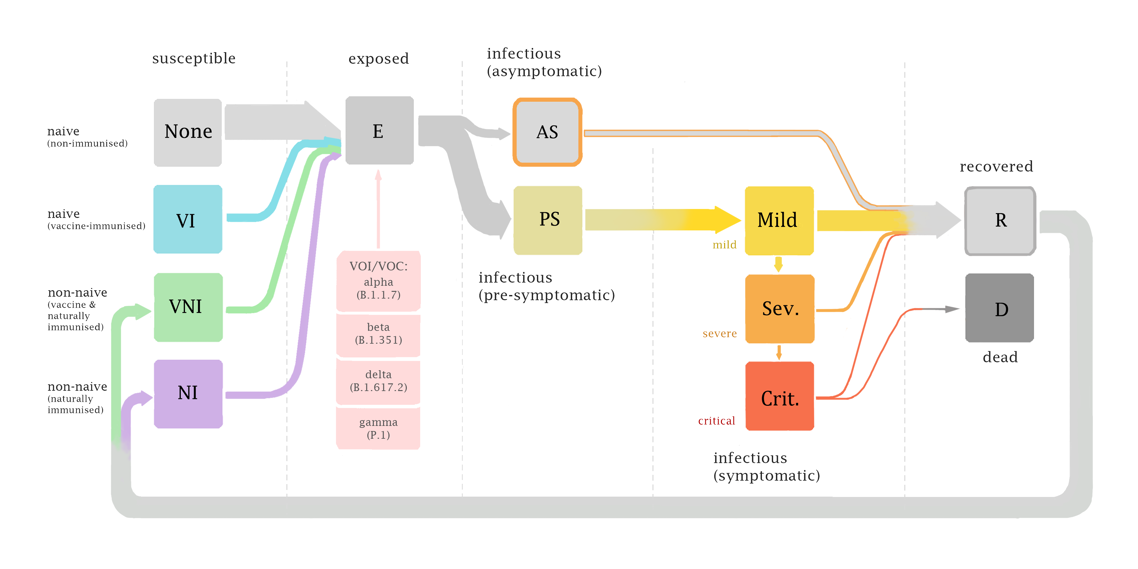
\includegraphics[width=1.0\textwidth]{figures/fig01_seir_v4 copy.png} 
    \caption{Schematic illustrating the mutually exclusive states agents can take in the model. Arrows denote direction of disease progression. Pink boxes denote variants of concern to which an agent can be exposed, and whose properties (e.g., such as transmissibility and severity) are already implemented in Covasim version 3.0.7 and above\cite{cohen2021mechanistic}. In this work, however, we only study the effects of the Alpha (B.1.1.7) and Delta (B.1.617.2) variants.}
\label{fig:covasim_qld_schematic}
\end{figure}

\subsection{Input Data}
The key empirical inputs to the model used in this work model include: 1) the composition of age and sex of the Queensland population; 2)  testing rates, tracing delays, and isolation and quarantine compliance (TTIQ) representative of the period February-October 2021; and, 3) the status of the vaccination rollout as of the middle of August 2021. The demographics of Queensland were taken from the 2016 census by the Australian Bureau of Statistics (ABS) (reference period September 2020). We do not include additional public health interventions (beyond TTIQ) such as short lockdowns, or layer-specific reduction in transmissibility due to mask wearing, so as to understand what would be the epidemic trajectories that could eventuate if any one variant of the virus is allowed to spread. We note that testing and contact tracing interventions used here (reflecting 2021 conditions) have changed with respect to the 2020 period for which the Queensland model was originally calibrated \cite{sanz-leon2021qldmodel}. The average number of daily tests increased from $\sim$ 6200 to $\sim$ 7500. This new baseline was estimated by calculating the mean number of tests between 15 February and 11 May 2021 using data from \url{https://covidlive.com.au/report/daily-tests/qld} -- last accessed 17 February 2022. The vaccination data used to determine the  ``incomplete'' status of the vaccine rollout (Fig.~\ref{fig:air_qld_vax_state}) were obtained from the daily reports from Australian Department of Health data. The vaccination rollout status on 17 August 2021 was the following: $\sim$ 43\% partially vaccinated people (having received at least one dose) and $\sim$ 25\% fully vaccinated people (having received two doses) over the age of 16, with lower rates for the young for whom access to vaccines began later. 

\begin{figure}[ht]
    \centering
    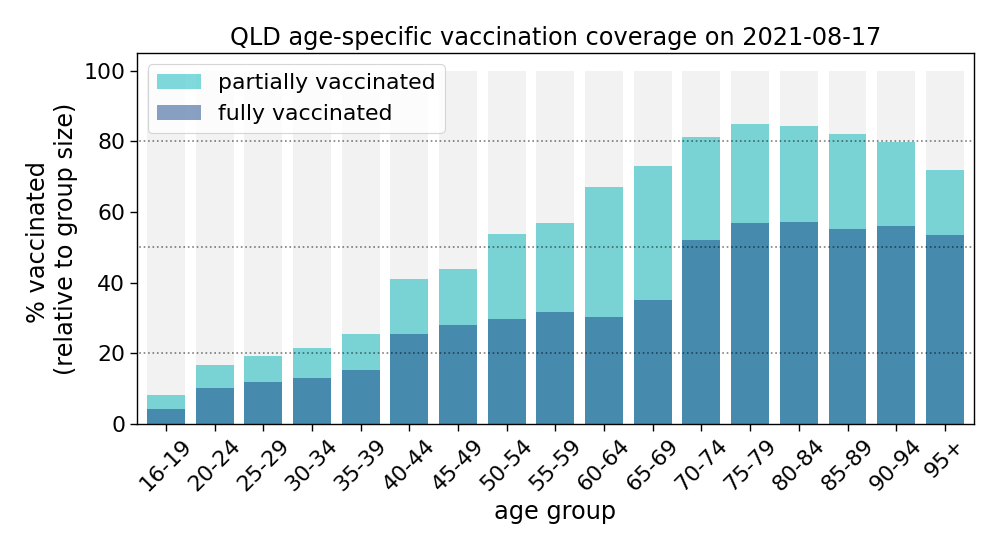
\includegraphics[width=0.8\textwidth]{figures/fig02_qld_vax_coverage_status_2021-08-17.png} 
    \caption{Age-specific state of vaccination in Queensland as of 17 August 2021. The height of each bar represents the percentage of people that have been either partially or fully vaccinated in that age group. Dotted lines indicate 20\%, 50\% and 80\%.}
    \label{fig:air_qld_vax_state}
\end{figure}

\subsection{General design of outbreak scenarios}
\label{subsec:design}

To determine whether herd immunity can be reached, we need to simulate outbreak scenarios. Using the calibrated Queensland model \cite{sanz-leon2021qldmodel}, we explored the impact of ``introduction scenarios'' in which a fixed  number infections were released into a population of 200,000 agents, a fraction of which has already been vaccinated. In all the scenarios presented here we infect 20 agents; this number of imports is all but guaranteed to generate sustained transmission without extinguishing by chance in the absence of further controls \cite{sanz-leon2021qldmodel}. The agents comprising the group of imported cases are drawn randomly and independently (i.e., they do not necessarily belong to the same household or workplace, though they could be related). This approach enables us to model scenarios such as an undetected leak from hotel quarantine (a common border control in Australia for much of the pandemic) or interstate travel, non-compliance with self-isolation, or separate undetected clusters in the community. A group of imported cases either has the Alpha variant or the Delta variant, but not a mix of both. 

All simulations included contact tracing (assuming no limit to the number of contacts traceable per day), testing, and an assumed near-perfect effectiveness of both domestic self-isolation and quarantine on every network, except the home network (see Table~\ref{table:layer-tqi-params}). As in previous work, we define quarantine as segregation of potentially infected agents (not to be confused with hotel quarantine) and isolation as segregation of confirmed (via testing) infected agents. When infected agents are detected via testing, they are put in isolation. As a secondary effect the contacts of confirmed cases are traced and tested (with higher priority than the general population). The exposed contacts are then quarantined while they wait for their test result. 

Covasim's default assumption is that the transmissibility of asymptomatic and symptomatic cases is the same. This assumption is based on the results presented by He et al. 2020 \cite{he2020relative}, where they did not find a statistically significant difference between transmissibility in symptomatic and asymptomatic cases.
Further, while people with symptomatic disease may have higher viral loads and thus be more infectious, people who are actively experiencing symptoms are also less likely to be going about their normal daily activities (even if they haven't been tested). We do not know the magnitude of either of these opposing effects, so by default leave the relative transmissibility of asymptomatic and symptomatic at 1. We used this same assumption for our simulations with Alpha, Delta and Omicron variants. 

\subsection{Modelling vaccination}
We modeled a range of levels of vaccine coverage, that is the \textit{vaccinated proportion}, representing different stages (or stalling points) of the vaccination rollout to the eligible population. Unless specified otherwise, the eligible population consists of people aged 16 and over to represent Queensland's eligible population in August 2021. In Australia, Pfizer was approved for children aged 12-15 on September 13th, 2021 \cite{pfizer_12_15} and for ages 5-11 on January 10th, 2022 \cite{pfizer_5_11}. We modeled vaccination as affecting individual immunity in two distinct ways, each approach highlighting the effects of vaccination as relevant to the question at hand. 

\paragraph{Simple vaccination model} The first approach to vaccination \cite{kerr2020covasim} is a simplified implementation that directly modulates the likelihood of becoming infected on contact with an infected individual, and blocks progression to symptomatic disease for people who are vaccinated and become infected. This approach has one vaccine parameter: vaccine effectiveness against infection, representing a reduction in the probability of acquiring an infection when a contact occurs with an infectious case. This vaccination model reflects the number of completed (two-dose) vaccine treatments assigned to randomly-selected members of the eligible population. We note that the vaccine’s protection against infection can be thought of as leaky \cite{abeysuriyaroadmap} not sterilising (i.e., it is not the case that 80\% effectiveness means that 80\% of vaccinated people have perfect protection and 20\% have no protection). Using this vaccine model each person vaccinated has reduced but non-zero risk of becoming infected based on the vaccine effectiveness, with the only exception to this rule being a vaccine effectiveness of 100\% which reduces the probability of acquiring an infection to 0. This vaccine model makes the additional assumption that people who are vaccinated and become infected will be 100\% protected from symptomatic disease, meaning they will no longer develop symptoms (both mild and severe) or progress into critical states and death (see Table~\ref{table:vax-params}). Another simplifying assumption of this model is that it does not explicitly model the reduction of onward transmission \cite{harris2021effect, pruna2022onward, creswell2022ptrsa-onwards}. We used the simple vaccine model in the simulated scenarios presented in \textit{Case 1a} in the next section, where we systematically explore the levels of protection against outbreak afforded by combinations of two parameters: vaccine effectiveness, and vaccine coverage (reported as a fraction of the eligible population vaccinated). 

\paragraph{Realistic vaccination model} The second approach to vaccination  \cite{cohen2021mechanistic} moderates the each agent's relative susceptibility to infection, to developing symptoms (i.e., asymptomatic vs symptomatic), and to severity of symptoms (pre-symptomatic, mild, severe needing hospitalization, and critical needing intensive care). This approach also accounts for protection against infection, protection against onward transmission ($\sim40$\% \cite{harris2021effect, pruna2022onward}), protection against symptomatic disease, and protection against severe disease \cite{cohen2021mechanistic} (see Table~\ref{table:vax-params}). Further, with this vaccination approach it is possible to have agents that have received only one dose (i.e., a partial vaccine treatment), and agents that have been vaccinated with two doses (i.e., a full vaccine treatment). The ideal interval between receiving the first and second dose is determined by the vaccine brand. The most important feature of this second approach is that it uses a detailed mechanistic model of immunity \cite{cohen2021mechanistic}, therefore it can also account for waning vaccine effectiveness over time; i.e., the decay in relative susceptibility to infection due to a decay in neutralising antibody concentration following vaccination. We employed this vaccination model for the scenarios presented in \textit{Case 1b} in the next section, where we systematically assess whether herd immunity is achieved for combinations of two parameters: partial versus full vaccination coverage; and in \textit{Case 2} where we assess the effect of age-specific hesitancy in health outcomes. In \textit{Case 1b} and \textit{Case 2} all vaccinated agents received the Pfizer--BioNTech vaccine, and waning immunity was accounted for. 

In this realistic vaccine model \cite{cohen2021mechanistic} protective efficacy is modelled as a function of neutralizing anitbodies (NAbs) \cite{khoury2020measuring}. Naive individuals are assumed to have no protective neutralizing antibodies against SARS-CoV-2. Upon vaccination or infection individuals draw an initial NAb level from a log-normal distribution, following the distribution used in Khoury et al. (2021) \cite{khoury2020measuring}. For vaccine-induced immunity, the specific parameters of this distribution depend on the vaccine administered and have been reported in Cohen et al. 2021 \cite{cohen2021mechanistic}. The key assumptions underlying NAbs kinetics are the following: NAbs grow linearly until they reach their peak after 3 weeks and then follow a two-part exponential decay, with a 100 day half-life in the first 250 days and an exponentially decaying decay rate until a 10-year half life is achieved \cite{cohen2021mechanistic, khoury2020measuring}. The implementation in Covasim allows for customisation of the functional form of the immunity kinetics, but because this is not the main focus of this work, we assume all individuals have the same kinetics for naturally-acquired and vaccine-induced immunity.  

\subsection{Modelling hesitancy}
Hesitancy is not uniform across age groups, with increased hesitancy in the young, as verified from survey data collected from Australian participants in August 2020, January 2021 and April 2021 \cite{biddle_change_2021} (Fig.~\ref{fig:hesitancy_per_age}). Indeed, between August 2020 and January 2021 hesitancy increased for all age groups but with a much larger increase for young adults than for the elderly. Thus, we modelled the effects of age-specific hesitancy by first selecting the proportion of agents who are hesitant, and leaving them unvaccinated for the course of the simulation. We used empirical data on hesitancy stratified by age \cite{biddle_change_2021}, and generated high, low, and optimistic hesitancy levels derived from observed variability between August 2020 and January 2021. In addition, we  investigated whether the age structure of hesitancy matters beyond the overall level of hesitancy, by setting the level of hesitancy to be homogeneous across all age groups.

\begin{figure}[ht]
    \centering
    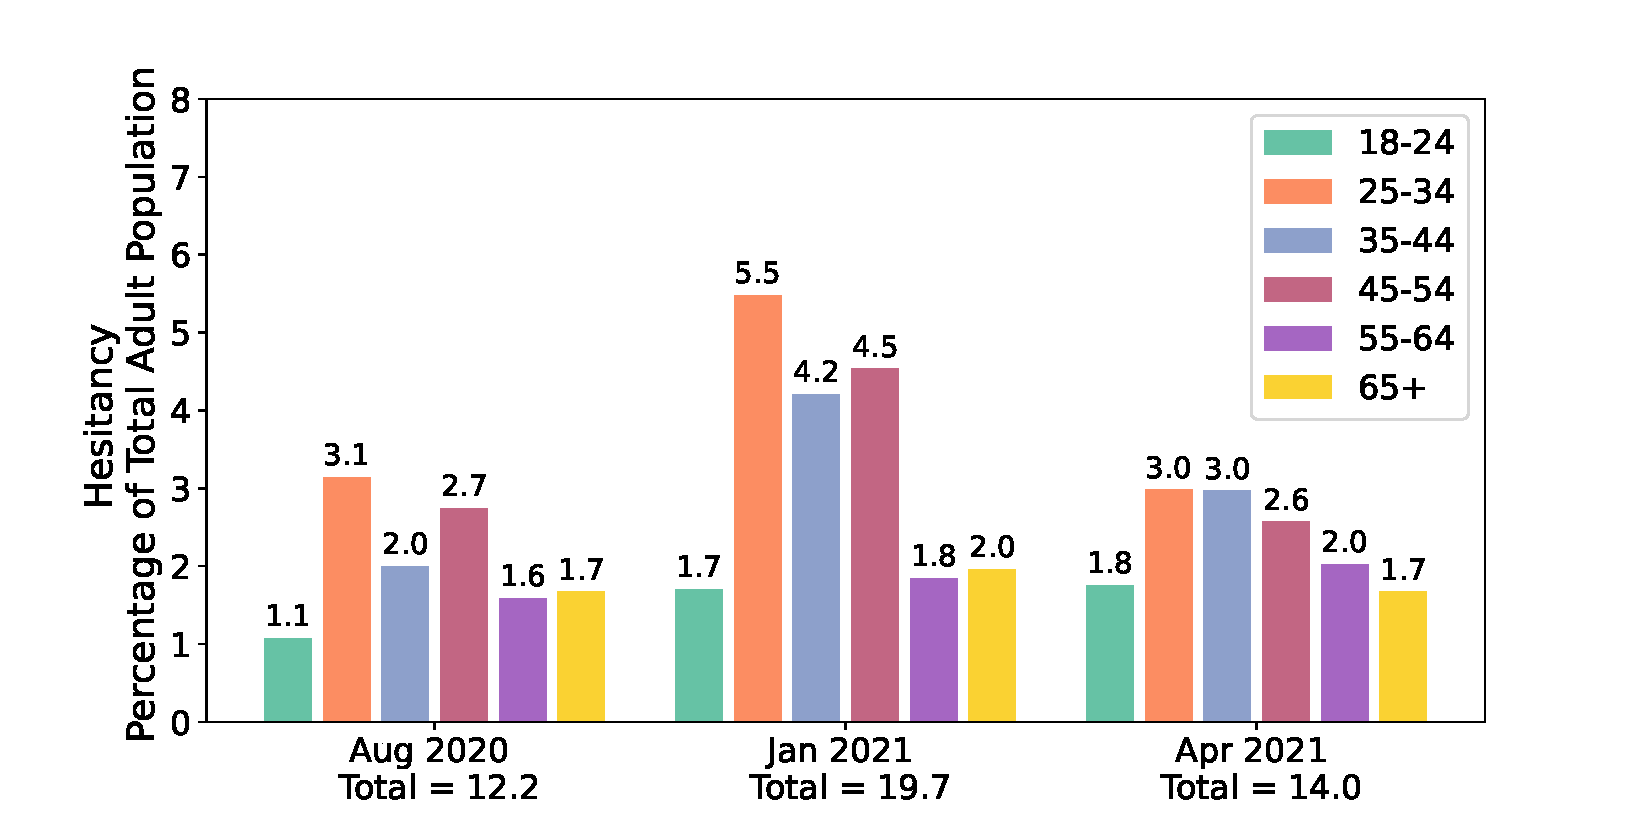
\includegraphics[width=0.65\textwidth]{figures/fig03_Hesitancy_Spec_vs_NonSpec.pdf} 
    \caption{Empirical Australian hesitancy rates in the adult population \cite{biddle_change_2021} in August 2020, January 2021 and April 2021, for six representative age groups. In this plot, the height of each bar is the hesitancy rate of a specific age group, and its value is expressed as a percentage relative to the size of the total adult population (i.e., aged 18 years and over).}
    \label{fig:hesitancy_per_age}
\end{figure}

\subsection{Assessing herd immunity and health outcomes}
\label{subsec:metrics}
To assess whether the population has achieved herd immunity or not, we used the effective reproductive number ($r_\mathrm{eff}$). This number encompasses the (average) number of secondary cases per infectious case in a population with multiple levels of susceptibility and/or immunity (derived naturally following infection or from vaccination). In Covasim the default method for computing $r_\mathrm{eff}$ is
\begin{equation}
r_{\mathrm{eff}}(t) = \frac{I_{n}(t)}{I_{a}(t)}\,w(t), 
\end{equation}
where $I_{n}(t)$ is the number of new infections on day $t$, divided by $I_{a}(t)$, the number of actively infectious people on day $t$, and multiplied by the mean duration of infectiousness $w(t)$. These instantaneous $r_\mathrm{eff}$ estimates are smoothed using a 7-day window.  

% Why did we choose reff30
The control threshold of $r_\mathrm{eff}=1$ is used to assess whether herd immunity has been achieved or not. If $r_\mathrm{eff}>1$, the number of new infections is increasing and if $r_\mathrm{eff} < 1$ there will be a decline in the number of new infections and the spread will eventually stop. Because we want to capture the undiluted effectiveness of vaccination interventions,  $r_\mathrm{eff}$ needs to be measured within a period where herd immunity has not been reached through widespread naturally acquired immunity. Further, we also take into account other practical considerations to narrow down the date on which we would assess herd immunity. For instance, within the first week of a simulation, $r_\mathrm{eff}$ estimates may have fluctuations \cite{li2022ptrsa-estimation} because of the underlying transient dynamics of the model, and the padding used for smoothing $r_\mathrm{eff}$ \cite{ackland2022ptrsa-fitting}. Thus we did not consider the first week as a suitable assessment period. We also let the epidemic trajectory evolve a further two weeks to account for the 
the delays in becoming infectious, symptom onset, and reporting. After all, $r_\mathrm{eff}$ at time $t$ still reflects transmission events from some time in the past.
Based on these considerations and preliminary results, we picked an observation window between days 21 and 35 where $r_\mathrm{eff}(t)$ was relatively constant or its derivative is close to 0  -- see Supp.~ Fig.~\ref{sup:fig:reff_timeseries}). Thus, for each simulation we extracted the value of $r_\mathrm{eff}$, 30 days after introducing 20 infected agents carrying a particular variant, either Alpha, Delta or Omicron, but not a mix of them. In the figures in Sec.~\ref{sec:results} we present the mean of this value, averaged across 1000 simulations, and simply denoted as $r_\mathrm{eff}^{30}$. 

%  How do we define the ranges
To assess herd immunity in Sec.~\ref{sec:results}-- \textit{Case 1a} and \textit{Case 1b} we define Queenslands's critical vaccination threshold to be the fraction of the eligible population that needs to be fully vaccinated so that $r_\mathrm{eff}^{30}=1$. However, to account for the uncertainty across the finite samples of 1000 simulations each, we determine a range of thresholds by defining bounds using the standard error in $r_\mathrm{eff}^{30}$ ($SE_\mathrm{r_\mathrm{eff}^{30}}$ shown for every scenario of \textit{Case 1a} in Supp.~Fig.~\ref{sfig:heatmap_plot_reff_SEMs}). Therefore, the range of critical vaccination thresholds encompasses vaccine coverage values between: (1) the highest vaccine coverage level for which $r_\mathrm{eff}^{30} - SE_\mathrm{r_\mathrm{eff}^{30}} > 1$ (upper coverage bound); and, (2) the lowest coverage level for which $r_\mathrm{eff}^{30} + SE_\mathrm{r_\mathrm{eff}^{30}} < 1$ (lower coverage bound). 

To assess the effect of hesitancy in Sec.~\ref{sec:results}-- \textit{Case 1a}, we consider the cumulative number of deaths, the cumulative number of infections, and critical cases (used as a proxy of intensive care unit (ICU) occupancy) as representative health outcomes to be minimised. 
We report these quantities in the form of boxplots to give a an overview of typical values and  the uncertainty in each scenario.   


\section{Results}
\label{sec:results}
% In this section we present our main results regarding herd immunity attainability and the impact of hesitancy on potential health outcomes should an outbreak eventuate before reaching herd immunity. 

\subsection{Case 1: What are the requirements for Queensland to reach herd immunity?}
\label{subsec:case_i}
% Assuming the vaccination operates as improving transmission blocking and no immunity waning}. TL;DR we used cv.simple_vaccine()
\subsubsection*{Case 1a: Impact of protection against infection, and blocking symptomatic covid using a simple vaccination model.}
\label{subsubsec:1a}

% eligible pop 16+ 
We examined the combined effect of vaccine coverage and vaccine effectiveness (protection against infections) on outbreaks where only one of the main variants (Alpha, Delta and Omicron) was dominant. With the eligible population restricted to ages 16+, we found that reliably controlling outbreaks is substantially more difficult for Delta than Alpha (Fig.~\ref{fig:heatmap_plot_reff}A and C), and unrealistic for Omicron (Fig.~\ref{fig:heatmap_plot_reff}E). Reliably achieving herd immunity (with TTIQ in place) against the Alpha variant requires vaccine effectiveness $\ge$80\% with $\ge$60\% coverage of the eligible population (48\% of the total population), and $\ge$50\% coverage (40\% of total) for 90\% effectiveness. Against the Delta variant herd immunity is only reliably achieved for a vaccine effectiveness $\ge$ 90\%, and requires $\ge$90\% vaccination coverage of the eligible population (i.e., $\sim$ 72\% of the total population). Herd immunity can only be achieved against the Omicron variant if the vaccine provides 100\% protection against infection, and $\ge$ 90\% of the eligible population is vaccinated ($\ge$ 72 \% of the total population). The values we just mentioned are the upper bounds of requisite vaccination coverage, which show the lowest level of uncertainty (i.e., more than 50\% of the simulations have $r_{\mathrm{eff}}^{30} < 1$ as shown in Supp.~Fig.~\ref{sfig:heatmap_plot_reff_proportions}).  

% eligible pop 12+
We repeated these scenarios for an expanded eligible population including individuals aged 12 years old and over (which occurred in Queensland in September 2021) (Fig.~\ref{fig:heatmap_plot_reff}B, D and F). These results show herd immunity may be achieved against Alpha for a vaccine coverage as low as $\sim$40\% of the eligible population ($\sim$ 34\% of the total population), assuming a vaccine effectiveness of at least 90\%. Against Delta herd immunity may be achieved for a vaccine effectiveness of at least 80\%, and vaccine coverage of 80\% of the eligible population ($\geq$ 68\% of the total population). Herd immunity is not attainable against Omicron unless the vaccine effectiveness is at least 90\%, and 90\% of the population aged 12 and older is vaccinated ($\sim$77\% of the total population).

% eligible pop 0+
We also repeated these scenarios when the entire population is eligible (Supp.~Fig.~\ref{sup:fig:heatmap_plot_reff} -- mean $r_{\mathrm{eff}^{30}}$;  Supp.~Figs~\ref{sup:fig:heatmap_plot_reff_sem}--\ref{sup:fig:heatmap_plot_reff_proportion} -- uncertainty measures of $r_{\mathrm{eff}}^{30}$). These results are consistent with those of an eligible population aged 12 and older: for a vaccine with 90\% effectiveness against the Alpha variant $\sim$ 35\% of the total population would need to be vaccinated. For a vaccine with 90\% effectiveness against Delta $\ge$ 50\% of the population would need to be vaccinated. Herd immunity can also be achieved against the Omicron variant with a 90\% effective vaccine if $\ge$ 70\% of the population is vaccinated, slightly lower than both the 90\% eligible and 77\% total population required if only ages 12 and up are vaccinated. These results support the idea that the expansion of the vaccination program can have a marked qualitative impact on the dynamics of the spread against Omicron. 

% Secondary effect of silent spreaders
As a secondary effect, we note that for low vaccine effectiveness the $r^{30}_\mathrm{eff}$ values increase for increasing coverage (top right corner of Figs~\ref{fig:heatmap_plot_reff}A-D). This is because this simplified vaccine model has perfect protection against symptomatic disease, which interacts with differential testing rates for asymptomatic and symptomatic individuals. In essence, this models the effect of ``silent spreaders'', overconfident that they are protected and less likely to test. 

% Move table to this section 
Table \ref{table:results-herd-immunity-threshold} summarises the critical levels of vaccination needed in Queensland for practical herd immunity against the Alpha or Delta variants (maintaining testing, testing, and isolation measures), for values of vaccine effectiveness against infection $\geq$ 80\%
and all three eligible populations shown in Fig.~\ref{fig:heatmap_plot_reff} and Supp.~Fig.~\ref{sup:fig:heatmap_plot_reff}. 

\begin{table}[h]
\begin{center}
\begin{tabular}{ |c|c|c|c| }
 \hline
  \textbf{Vaccine effectiveness} & \multicolumn{3}{|c|}{\textbf{Eligible population}} \\
  \hline
 \cellcolor[HTML]{EFEFEF}{\textbf{0.8 (80\%)}} &  \cellcolor[HTML]{EFEFEF}{\textbf{16+}} &  \cellcolor[HTML]{EFEFEF}{\textbf{12+}} &  \cellcolor[HTML]{EFEFEF}{\textbf{0+}} \\
 \hline
Alpha                     & 50\% - 60\% & 40\% - 60\% & 35\% - 45\% \\ 
\hline
Delta                     & N/A         & 70\% - 80\%    & 60\% - 65\%      \\
\hline
Omicron                  & N/A          & N/A      &    85\% - 90\%       \\
\hline
 \cellcolor[HTML]{EFEFEF}{\textbf{0.9 (90\%)}}& \cellcolor[HTML]{EFEFEF}{\textbf{16+}} &  \cellcolor[HTML]{EFEFEF}{\textbf{12+}} &  \cellcolor[HTML]{EFEFEF}{\textbf{0+}} \\
\hline
Alpha                    & 30\% - 50\% & 30\% - 40\%  &  30\% - 35\%\\
\hline
Delta                    & 70\% - 80\% & 50\% - 70\%  &  50\% - 55\% \\
\hline
Omicron                  & N/A & 80\% - 90\% &  65\% - 70\% \\
\hline
 \cellcolor[HTML]{EFEFEF}{\textbf{1.0 (100\%)}}& \cellcolor[HTML]{EFEFEF}{\textbf{16+}} &  \cellcolor[HTML]{EFEFEF}{\textbf{12+}} &  \cellcolor[HTML]{EFEFEF}{\textbf{0+}} \\
\hline
Alpha                    & 30\% - 50\% & 30\% - 50\%  &  25\% - 30\%\\
\hline
Delta                    & 50\% - 60\% & 40\% - 60\%  &  40\% - 45\% \\
\hline
Omicron                  & 80\% - 90\% & 60\% - 70\% &  55\% - 60\% \\
\hline
\end{tabular}
\caption {Critical vaccination threshold ranges necessary to reach herd immunity in Queensland against Alpha, Delta and Omicron, given vaccine effectiveness of 80\%, 90\% or 100\%. N/A means herd immunity is not achieved.} 
 \label{table:results-herd-immunity-threshold}
\end{center}
\end{table}

\begin{figure}[H]
    \centering
    \sidesubfloat[]{\label{fig:heatmap_plot_reff:sub:a:b117-16}\includegraphics[width=0.45\textwidth]{figures/fig04a_results_vax-heatmap_Mean_alpha_16yo-cs20-reff30_Apr2022.png}}
    \hfill
    \sidesubfloat[]{\label{fig:heatmap_plot_reff:sub:b:b117-16}\includegraphics[width=0.45\textwidth]{figures/fig04b_results_vax-heatmap_Mean_alpha_12yo-cs20-reff30_Apr2022.png}}
    \hfill
    \sidesubfloat[]{\label{fig:heatmap_plot_reff:sub:c:b16172-16}\includegraphics[width=0.45\textwidth]{figures/fig04c_results_vax-heatmap_Mean_delta_16yo-cs20-reff30_Apr2022.png}}
    \hfill
    \sidesubfloat[]{\label{fig:heatmap_plot_reff:sub:d:b16172-16}\includegraphics[width=0.45\textwidth]{figures/fig04d_results_vax-heatmap_Mean_delta_12yo-cs20-reff30_Apr2022.png}}
    \hfill
    \sidesubfloat[]{\label{fig:heatmap_plot_reff:sub:e:ba1-12}\includegraphics[width=0.45\textwidth]{figures/fig04e_results_vax-heatmap_Mean_omicron_16yo-cs20-reff30_Apr2022.png}}
    \hfill
    \sidesubfloat[]{\label{fig:heatmap_plot_reff:sub:f:ba1-16}\includegraphics[width=0.45\textwidth]{figures/fig04f_results_vax-heatmap_Mean_omicron_12yo-cs20-reff30_Apr2022.png}}
    \hfill
    \caption{Effective reproductive number 30 days after seeding an outbreak ($r^{30}_\mathrm{eff}$), as a function of vaccine effectiveness (infection blocking) and vaccine coverage (fraction of the eligible population vaccinated, shown along the top axes). The fraction of the total population vaccinated is shown along the bottom axes. Outlined areas indicate values of vaccine coverage over which herd immunity is reached as per the definition given in Sec.~\ref{subsec:metrics} for those vaccine effectiveness values at which herd immunity is achieved at all. We have clipped the colour scale such that $r^{30}_\mathrm{eff} \in$ [0.5, 1.5] to better see the zone near $r^{30}_\mathrm{eff}=1$. \textbf{A:} Alpha variant, ages 16+ eligible. \textbf{B:} Alpha variant, ages 16+ eligible. \textbf{C:} Delta variant, ages 16+ eligible. \textbf{D:} Delta variant, ages 12+ eligible. \textbf{E:} Omicron variant, ages 16+ eligible. \textbf{F:} Omicron variant, ages 12+ eligible.
    Initial number of imported infections is 20, other simulation parameters are summarized in Supp. Table~\ref{table:herd-model}.}
    \label{fig:heatmap_plot_reff}
\end{figure}

\begin{figure}[H]
    \centering
    \sidesubfloat[]{\label{fig:heatmap_plot_reff_first_second:sub:a:16}\includegraphics[width=0.7\textwidth]{figures/fig05a_results_vax-heatmap_full-partial_Mean_delta_16yo-cs20-reff30_Feb2022.png}}
    \hfill
    \sidesubfloat[]{\label{fig:heatmap_plot_reff_first_second:sub:b:12}\includegraphics[width=0.7\textwidth]{figures/fig05b_results_vax-heatmap_full-partial_Mean_delta_12yo-cs20-reff30_Feb2022.png}}
    \hfill
    \caption{Partial versus full vaccination coverage. Effective reproductive number on day 30 after initial infections are imported ($r^{30}_\mathrm{eff}$), as a function of the proportion of people that received at least one dose and the proportion of people who received two doses (everyone receives Pfizer and the proportions along the top axis are with respect to the eligible population. In all scenarios 20 agents infected with the Delta variant are inserted into the community. We have clipped the colour scale such that $r^{30}_\mathrm{eff} \in$ [0.5, 1.5] to better see the zone near $r^{30}_\mathrm{eff}=1$. \textbf{A}: Eligible population 16+. \textbf{B:} Eligible population 12+. From top left to bottom right, the yellow squares illustrate the progression of the vaccine rollout in Queensland, from top-left to bottom-right, starting from August 1st 2021 and proceeding  along the first of each month through to January 2022 \cite{air_vax_data}.}
    \label{fig:heatmap_plot_reff_first_second}
\end{figure}

\begin{figure}[H]
    \centering
    \sidesubfloat[]{\label{fig:heatmap_plot_reff_first_second_omicron:sub:a:16}\includegraphics[width=0.7\textwidth]{figures/fig06a_results_vax-heatmap_full-partial_Mean_omicron_12yo-cs20-reff30_Feb2022.png}}
    \hfill
    \sidesubfloat[]{\label{fig:heatmap_plot_reff_first_second_omicron:sub:b:12}\includegraphics[width=0.7\textwidth]{figures/fig06b_results_vax-heatmap_full-partial_Mean_omicron_16yo-cs20-reff30_Feb2022.png}}
    \hfill
    \caption{Partial versus full vaccination coverage. Effective reproductive number on day 30 after initial infections are imported ($r^{30}_\mathrm{eff}$), as a function of the proportion of people that received at least one dose and the proportion of people who received two doses (everyone receives Pfizer and the proportions along the top axis are with respect to the eligible population. In all scenarios 20 agents infected with the Omicron variant are inserted into the community. We have clipped the colour scale such that $r^{30}_\mathrm{eff} \in$ [0.5, 1.5] to better see the zone near $r^{30}_\mathrm{eff}=1$. \textbf{A}: Eligible population 16+. \textbf{B:} Eligible population 12+. From top left to bottom right, the yellow squares illustrate the progression of the vaccine rollout in Queensland, from top-left to bottom-right, starting from August 1st 2021 and proceeding  along the first of each month through to January 2022 \cite{air_vax_data}.}
    \label{fig:heatmap_plot_reff_first_second_omicron}
\end{figure}

\subsubsection*{Case 1b: Impact of different coverage rates of single versus double doses using a realistic vaccination model}
\label{subsubsec:1b}

We next asked whether vaccine rollouts with supply constraints should target the completion of second doses or aim for maximal first dose coverage first. We simulated scenarios where we vaccinated a proportion of people with only one dose (partial vaccination), and a proportion of people with two doses (full vaccination). In these scenarios everyone received Pfizer doses, and coverage values are with respect to the eligible population. Vaccine efficacy values used in these scenarios are presented in Supp. Table~\ref{table:vax-params}. We found that very high ``at least one  dose coverage'' ($>95\%$) confers substantial protection against infection with $r_\mathrm{eff}^{30} \approx 1$ even for low rates of ``two doses'' coverage ($<30\%$), for eligible populations 16+ (Fig.~\ref{fig:heatmap_plot_reff_first_second:sub:a:16}) and 12+ (Fig.~\ref{fig:heatmap_plot_reff_first_second:sub:b:12}). 

Using the definition of herd immunity given in Sec.~\ref{subsec:metrics} we find that for an eligible population 16+, if 100\% received at least one dose, herd immunity could be achieved if 25\% - 45\% of the eligible population receive two doses. On the other hand, if 100\% of an eligible population 12+ received at least one dose, herd immunity would be achieved a lower and a narrower two-dose coverage of 0\% - 20\% 

We also repeated these scenarios for the Omicron variant, for eligible populations 16+ (Fig.~\ref{fig:heatmap_plot_reff_first_second_omicron:sub:a:16}) and 12+ (Fig.~\ref{fig:heatmap_plot_reff_first_second_omicron:sub:b:12}). These results show that even with a high proportion ($>$95\%) of the eligible population receiving at least one dose, a high proportion of the eligible population should receive two doses to achieve herd immunity: 85\%-95\% (eligible pop. 16+) and 55\%-85\% (eligible pop. 12+). These results are consistent with what occurred in Queensland between December 2021 and January 2022. The proportion of the eligible population 16+ who had received two doses was below 80\% and put the population in a situation where an outbreak was inevitable. Uncertainty measures of $r_{\mathrm{eff}}^{30}$) for the scenarios presented in Figs \ref{fig:heatmap_plot_reff_first_second} and \ref{fig:heatmap_plot_reff_first_second_omicron} are provided in the Supp. Material in Figs \ref{sfig:heatmap_plot_first_second_sem}-\ref{sfig:heatmap_plot_reff_first_second_proportions}, and Figs \ref{sfig:heatmap_plot_first_second_sem_omicron}-\ref{sfig:heatmap_plot_reff_first_second_proportions_omicron}, respectively.  


Our results in Figs \ref{fig:heatmap_plot_reff_first_second} and \ref{fig:heatmap_plot_reff_first_second_omicron} show that prioritization of two-dose vaccination (i.e., moving down the diagonal instead of moving to the right), would result in minimal reductions in $r_\mathrm{eff}^{30}$. These results indicate that administering first doses should be prioritised regardless of the minimal age included in the vaccination program. However, to control outbreaks by bringing $r_\mathrm{eff}^{30}<1$ with TTIQ alone requires administration of second doses---particularly since the 95\% at least one-dose coverage above has proven to be difficult to attain in Queensland. 


\subsection{Case 2: How does vaccine hesitancy affect health outcomes in Queensland?}
\label{subsec:case_ii}
% What we did here
We next examined scenarios with realistic age-dependent hesitancy rates and the realistic vaccine model (see Supp.~Table~\ref{table:Hesitancy_Parameters_Months} for a breakdown of these values by age group). We simulated outbreaks of the Delta variant with TTIQ as the only intervention and observed the resulting epidemic trajectories. We first note that herd immunity was not reached in most of these simulations (i.e., $r_{eff}^{30}>1$ and large outbreaks occur, albeit occasionally delayed by initial slow growth in a highly vaccinated population). To assess disease severity and burden, in each each scenario we quantified infections, critical cases, and deaths. We also chose to report cumulative results at 90 days as our cutoff, as these key indicators take time to accumulate.


% Eligible pop 16+ - low (april) and high (january) points of hesitancy
We asked whether the observed fluctuations in age-specific hesitancy levels in Australia (Fig.~\ref{fig:hesitancy_per_age}) would have a significant effect on health outcomes, assuming that these hesitant proportions represent the final unvaccinated populations. We used values from January 2021 (19.7\%) and April 2021 (14.0\%), which were representative high and low points during the first half of 2021. We henceforth refer to these levels of hesitancy as ``high'' and ``low''.   
With the delta variant, the change from ``high'' hesitancy to ``low'' hesitancy manifests in all age categories as lower numbers of infections, critical cases, and deaths (Fig.~\ref{fig:AgeSpec_Hes_Outcomes_delta}A-B). While the $r_\mathrm{eff}^{30}$ mean values and standard deviation were similar for the ``high'' and ``low'' hesitancy scenarios (e.g., $1.5\pm0.7$ and $1.4\pm0.8$, respectively), small differences in exponential growth rate can manifest as large differences in health outcomes after 90 days. The largest difference in health outcomes was a 52\% decrease in number of infected people aged 25--34 (attributable to the particularly large difference in hesitancy among the young), and 43\% decrease in the number of deaths for the vulnerable 65+ group. This demonstrates that a drop from $\sim$20\% to $\sim$14\% in overall hesitancy---with larger drops in the hesitant young---can have a relatively large positive effect on lives saved and burden of disease.
 

% Eligible pop 16+ and non-specific hesitancy supp mat
To confirm that the age structure makes a difference beyond simply the overall rates of hesitancy, we compared health outcomes between the empirical age distributions and surrogate distributions with constant non-specific hesitancy (Supp. Fig.~\ref{sfig:FiguresCompare_AgeSpec}). This comparison shows that the total number of infections remain similar (with decreases in youthful population and increases in older population), but the age structure contributes to substantial differences in deaths and critical cases. Non-specific hesitancy yields up to 43\% more deaths than age-specific hesitancy, hence the age structure influences outcomes beyond simply the total vaccination coverage.

% Eligible pop 12+ - low and very low 
We next expanded the eligible population to include individuals aged 12 and over, and simulated two additional scenarios with plausible hesitancy levels. The first scenario assumed the ``low'' hesitancy level (14.0\%). Agents aged 12--16 were assigned the same hesitancy as the 35--44 group, which we assumed to be their parents (Fig.~\ref{fig:AgeSpec_Hes_Outcomes_delta}C). The second scenario set hesitancy homogeneously across all age groups to 8\%, which was the lowest observed hesitancy of any age-group in April 2021 (Fig.~\ref{fig:AgeSpec_Hes_Outcomes_delta}D), and henceforth referred to as ``very low''.  We note that these scenarios fell within the region where herd immunity could be attained for the delta variant. Their delta $r_\mathrm{eff}^{30}$ mean values and standard deviation were $1.0\pm0.8$ and $0.9\pm0.7$, for the ``low'' and ``very low'' hesitancy scenarios, respectively.   

% Comparing stuff
A qualitative comparison between the health outcomes of the scenario with 16+ eligibility and ``low'' hesitancy (Fig.~\ref{fig:AgeSpec_Hes_Outcomes_delta}C) and the two 12+ eligibility scenarios with ``low'' and ``very low'' hesitancy (Fig.~\ref{fig:AgeSpec_Hes_Outcomes_delta}B--D), reveals that in the latter two, there is a reduction by more than half in the cumulative number of infections, critical cases, and deaths in all age-categories. Expanding the eligible population to include the 12--15 age group reduced the median number of infections in the 0--14 and 15--24 age group by over 75\%, and by a further 60\% if all age groups can reach the vaccination rates of the oldest group (``very low'' hesitancy). Large improvements were also seen outside of this age-group, with vaccination of 12--15 year olds reducing the median number of deaths in the 65+ group by 77\%, and by a further 66\% for ``very low'' hesitancy case.

\begin{figure}[]
    \centering
     \sidesubfloat[]{\label{sfig:CombinedAgeSpecJanuaryDelta_AgeSpec_ClusterSize_20}\includegraphics[width=0.45\textwidth]{figures/fig07a_January2021_delta__BoxPlot_AgeSpec_Day_90.jpg}}
    \hfill
      \sidesubfloat[]{\label{sfig:CombinedAgeSpecAprilDelta_AgeSpec_ClusterSize_20}\includegraphics[width=0.45\textwidth]{figures/fig07b_April2021_delta__BoxPlot_AgeSpec_Day_90.jpg}}
    \hfill
 \sidesubfloat[]{\label{sfig:CombinedAgeSpecNoYouthHesDelta_AgeSpec_ClusterSize_20}\includegraphics[width=0.45\textwidth]{figures/fig07c_April_12_2021_delta__BoxPlot_AgeSpec_Day_90.jpg}}
     \hfill
 \sidesubfloat[]{\label{sfig:CombinedAgeSpecLowHesDelta_AgeSpec_ClusterSize_20}\includegraphics[width=0.45\textwidth]{figures/fig07d_LowHesitancy_delta__BoxPlot_AgeSpec_Day_90.jpg}}
    \caption{A comparison of age-specific health outcomes: infections (green), critical cases (red), deaths (grey), 90 days after the insertion of 20 agents infected with the Delta variant. \textbf{A:} Eligible population 16+, with age-specific hesitancy as in January 2021. \textbf{B:} Eligible population 16+, with hesitancy as in April 2021. \textbf{C:} Eligible population 12+, with hesitancy levels as in April 2021, and individuals aged 12-17 are assigned their parents' hesitancy (i.e., in the 35-44 bracket).  \textbf{D:} Eligible population 12+, and all agents have 8\% hesitancy, which is the lowest observed in empirical data across all age-groups. The values correspond to number of individuals in each state and age bin (boxplot of $1000$ simulations, with individual results overlaid), for all individuals (light coloured bars), and the vaccinated subset (dark coloured bars). The hesitancy and vaccination coverage are summarized in Supp. Table~\ref{table:Hesitancy_Parameters_Months}.}
    \label{fig:AgeSpec_Hes_Outcomes_delta}
\end{figure}


\section{Discussion}
\label{sec:discussion}

% Summary of what we did here
In this work, we aimed to (i) determine whether plausible combinations of vaccine effectiveness and vaccine coverage in Queensland allow the possibility of reaching herd immunity against the Alpha, Delta and Omicron variants, without widespread natural immunity; and, (ii) determine whether age-dependent variability in hesitancy, coupled to the population age structure, poses additional challenges for control of COVID-19 outbreaks. The main rationale was to understand whether vaccination and mild non-pharmaceutical interventions (TTIQ) would be sufficient to prevent outbreaks given the rise of new variants. We further expected that identifying age brackets that have the largest impact on health outcomes may help to guide strategies for boosting vaccine willingness in key demographics.

% A summary of our results
Our modelling results highlight how important it was that Queensland, and other settings with similar demographics and low natural immunity, vaccinate its population with high coverage. We identified practical critical vaccination thresholds for protection against the Alpha and Delta variants: for Alpha, only 48\% of the overall population is required to be vaccinated to drastically curb the number of deaths and infections, this lying at the upper edge of the range of critical thresholds; with the Delta variant, 48\% coverage lies at the lower edge of critical vaccination thresholds, and herd immunity can only be reliably achieved if 72\% of the total population is vaccinated. These Delta targets were only reached around the end of 2021, by which time the Omicron variant had already arrived. But in any case once we factor in waning of immunity---equivalent to weakening of vaccine effectiveness in our simulations---herd immunity cannot be reached. Hence Queensland is unlikely to be sufficiently protected against new incursions without additional health measures beyond TTIQ. This situation can only be worsened by waning compliance with control measures in the population as the pandemic drags on.

% A summary of our results about hesitancy and health outcomes
In terms of health outcomes, results comparing different levels of hesitancy demonstrated that a small drop in global hesitancy (from $\sim$ 20\% to $\sim$ 14\%), within the ranges that have been recorded in longitudinal surveys, can greatly reduce infections and deaths. Moreover, we showed that more extensive vaccination of the young can protect the elderly. Reducing hesitancy of the age 12--34~y population can greatly reduce deaths in older age brackets. Our results also support targeting high vaccine uptake among the group aged 12--15 years old; school-based programs may be beneficial to achieve this.  Further cross-interactions between age-specific hesitancy and different population demographics should also be investigated (for example, cross-interaction between age-specific hesitancy and use of social media; age-specific hesitancy and geographic location). It also remains to be seen how adult hesitancy will affect consent for their children to receive vaccines.

% Limitations of our work - vaccines
One limitation of this study is that we have not sought to model the roll-out trajectory itself, instead opting for the simpler case of examining the situation once the roll-out stalls upon vaccinating all of the (currently-projected) willing members of the population. We did, however, examine differences in $r_\mathrm{eff}$ between different rates of single versus double doses (which can be important \cite{bernal_delta_2021,voysey2021safety,williams_outbreak_2021}). We also simplified the mix of vaccines, modeling scenarios that assumed an overall level of vaccine effectiveness averaged across vaccine brands, and optimistic scenarios where all agents were vaccinated with Pfizer, whose effectiveness may be overstimated with respect to Omicron. In the Pfizer-only simulations, the waning effectiveness for all agents started at the same date -- creating a relatively homogeneous level of protection in different age-groups. The specific vaccine brands and their waning effectiveness in each age group is an area for future work. Our results spanning a range of effectiveness values (Fig.~\ref{fig:heatmap_plot_reff}) speak to possible waning scenarios: waning corresponds to reduced effectiveness and hence drifting upwards in the plotted grid. Rollout of vaccine booster doses can be considered as undoing waning, rapidly moving downward in the plotted grids. Likewise, the potential effects of new variants (e.g. Omicron and beyond) could be mapped out systematically by exploring different rates of vaccine escape and intrinsic transmissibility.

% NEW PARA: Limitations of our work: relaxing scenarios and single variant scenarios
Another simplification in our scenarios was the assumption only one variant was circulating at any time, rather than a mix of multiple variants. At the time this work was carried out, our assumption was supported by earlier modelling studies where it was shown that in settings like Queensland with near-zero prior naturally acquired immunity and no countermeasures in place, a more transmissible variant (like Omicron) rapidly outcompetes a less transmissible variant (like Delta) \cite{cohen2021mechanistic,ramos2021modeling, layton2022ontario}. This assumption was confirmed by the Omicron wave experienced in Queensland in January 2022. When Queensland reopened its interstate borders in the middle of December 2021, Delta was the prevalent variant in Australia, but by the end of December 2021 it was estimated that Omicron (BA.1) accounted for $\sim$84\% of infections \cite{qld-omicron-ba1-84}. Indeed BA.1 has since been usurped by BA.2 (as at May 2022), and there are other even more transmissible Omicron subtypes in circulation globally \cite{uk-hsa-may-2022}.

% another new one on limitations that may affect transmission dynamics
Other limitations that would likely affect the transmission dynamics include our assumption that TTIQ effectiveness does not reduce over time, which would reflect "fatigue" with restrictions in the community as well as the rolling back of this intervention (and indeed as of May 2022 contact tracing has largely ended in Queensland and close contacts no longer need to isolate in most cases). We also do not model seasonal or day-of-the-week effects on contact networks. And while we have incorporated a moderate degree of realism in our contact networks, there remains considerable uncertainty in their parameterisations, and particular high-risk settings (aged care, hospitals, and their workforces) are not explicitly modelled.

% NEW PARA: DEMOGRAPHIC TURNOVER
Beyond the short term, demographic changes could affect the course of the pandemic: changes in age distribution and household size and composition have been shown to be significantly associated with different rates of COVID-19 incidence and mortality \cite{karmakar2021association_us, mah2022social}. Given that Australia's large "baby boomer" generation is approaching the ages where risk of severe outcomes increases steeply, and coupled with waning immunity, concerted effort may be required to maintain immunity levels to prevent deterioration of health outcomes. Moreover, births supply a steady stream of new unvaccinated individuals faster than the death rate. While Australia has a generally high vaccination rate for children, and high coverage overall against COVID-19, only $\sim$40\% of Queensland children aged 5-11 have received their first dose as at May 2022. Sustained low coverage among children could thus erode total population vaccination coverage, though, in the end, the Omicron wave has conferred substantial immunity to the young.

% NEW PARA - onward transmission
In this work we have analysed the level of vaccine coverage and effectiveness to achieve herd immunity in a with low natural immunity, and while our model has been customised to the population of Queensland and incorporates a high degree of population heterogeneity (e.g., age-specific prognoses and immunity properties \cite{waites2022ptrsa-compositional}), there were many simplifying assumptions made in Sec.~\ref{sec:results} -- \textit{Case 1a}, including the lack of an explicit reduction in onward transmission. However, there is evidence showing that immunisation with either Pfizer \cite{harris2021effect,pruna2022onward} or AstraZeneca \cite{harris2021effect} reduces the chance of onward virus transmission by 40–60\%. For that reason, we introduced this effect into our more realistic scenarios Sec.~\ref{sec:results} -- \textit{Case 1b} and \textit{Case 2}. We notice that despite the absence of onward transmission effectiveness, the results in \textit{Case 1a} (Delta variant, eligible population 12+, and vaccine effectiveness of ~90\%) yield more optimistic estimates of herd immunity thresholds than those in \textit{Case 1b} (same variant, same eligible population). This is because in Covasim a reduction in the probability of developing symptoms results in a reduction in the relative transmissibility of individuals. Because our simple vaccination model provides a perfect protection against symptoms, not only does it counteract the absence of an explicit onward transmission effectiveness, but it likely overestimates the overall effect of vaccines on transmission.

% HOW DO OUR RESULTS COMPARE TO OTHERS
The results from our scenarios with Delta and Omicron, an eligible population encompassing the total population and vaccine effectiveness above 80\%, are consistent with estimates from earlier modelling work \cite{gomes2022individual, britton2020mathematical} where herd immunity thresholds sit at 60-70\% of the total population, assuming vaccines are delivered at random and (naive) individuals mix at random. However, it has also been shown that prior exposure to infection can lower the herd immunity thresholds to $\sim$40\% \cite{britton2020mathematical}. These modelling results are supported by retrospective observational studies reporting that previous infection with SARS-CoV-2 provides stronger and longer protection compared to vaccine-induced protection in naive individuals \cite{gazit2021comparing}. For Queensland, and similar settings, this indicates that the population may need to adopt frequent administration of boosters compared to other locations such as the UK \cite{gomes2022individual}. However, since the arrival of Omicron in December 2021, Queensland has experienced two waves of infections, with their peaks around the middle of January 2022 and early April 2022 respectively, with more waves expected during the winter season (March-August 2022) \cite{qld-omicron-peak-2}. This will confer the population additional protection acquired through infections. Preliminary results from Qatar estimated the protection gained from Omicron infection against future Omicron (symptomatic) reinfections is approximately 56\% \cite{altarawneh2022protection}. Thus the effective herd immunity thresholds of Queensland may be lower than the ones obtained in this study. 

% OUTLOOK   
Perhaps the most critical and outstanding question is: how do we maintain the state of herd immunity in the long run? Factoring in waning of immunity, which is equivalent here to drifting ``upwards'' in the heatmaps of Fig.~\ref{fig:heatmap_plot_reff}, implies that even if herd immunity were attained it would be a transient state in the absence of boosters.


\section{Conclusions}
\label{sec:conclusion}
In this paper, we have assessed the practicality of achieving herd immunity against the Alpha (B.1.1.7), Delta (B.1.617.2) and Omicron (BA.1) variants of SARS-CoV-2 in the state of Queensland, Australia---a region that until the end of 2021 had negligible rates of infection-acquired immunity, thus making our results a rare glimpse into herd immunity attained solely as the result of vaccination-induced immunity, rather than derived from prior infection -- or, a combination of both.  
Our simulations show that full herd immunity was unlikely to be achieved for the Delta and Omicron variant from currently-available vaccines alone. Assuming that vaccination provides, on average, an effectiveness of $\sim$90\% against infection---which is at the upper end of observed effectiveness \cite{pouwels2021vax_eff, ukhsa-vaccine-omicron}---extension of the vaccination program to children seems essential. Restricting eligibility to 16+ requires up to 90\% coverage, which proved in February 2022 to be near the maximum attainable given hesitancy rates, which should not be neglected. Indeed,  we have shown that small changes in vaccine hesitancy, which have occurred in Australia over short periods of time \cite{biddle_change_2021}, can have a large impact on the health outcomes for the entire population. 

% To use Vancouver style
\bibliography{corona-qld-vaccine}

\section*{Additional Information}

\medskip \noindent
All authors declare they have no conflict of interest. 

\section*{Data Availability}
The data used in this work is publicly available from \url{https://github.com/jxeeno/aust-govt-covid19-vaccine-pdf/blob/master/docs/data/air.csv}

\section*{Code Availability}
Code with the Queensland model, and data to reproduce the figures can be found here: 
\url{https://github.com/brain-modelling-group/paper-covid-herd-hesitancy}

\newpage
\appendix
% ############################ SUPP INFO ####################################
\section*{}

\begin{center}
    {\Large {Supplementary Information}}
    \vspace{1cm}
    
    Paula Sanz-Leon*, Lachlan H. W.  Hamilton, Sebastian J. Raison, Anna J. X. Pan, Nathan J. Stevenson, Romesh G. Abeysuriya, Robyn M. Stuart, Cliff C. Kerr, Stephen. B. Lambert and James A. Roberts.
\end{center}


\section{Supplementary Tables}
\setcounter{page}{1}
\renewcommand{\tablename}{Supplementary Table}
\renewcommand{\thetable}{S\arabic{table}}
\setcounter{table}{0}

Table~\ref{table:general-info} summarizes the references for the most relevant categories of parameters. When no precedent in the literature could be found for a particular parameter, a Delphi procedure (asking a panel of experts) was previously used to provide estimates \citep{kerr2020covasim,scott2020modelling}.

% General table - kinda index for supp tables
\begin{table}[h]
\begin{tabular}{|
>{\columncolor[HTML]{EFEFEF}}c |
>{\columncolor[HTML]{FFFFFF}}c |}
\hline
\multirow{2}{*}{\cellcolor[HTML]{EFEFEF}{\parbox{9cm}{\centering\textbf{Parameter}}}}    & 
\multirow{2}{*}{\cellcolor[HTML]{EFEFEF}{\parbox{4cm}{\centering\textbf{Source/Value}}}} \\ [4ex]
\hline
\multirow{2}{*}{\cellcolor[HTML]{FFFFFF}{\parbox{9cm}{\centering{Covasim version}}}}    &  
\multirow{2}{*}{\cellcolor[HTML]{FFFFFF}{\parbox{4cm}{\centering{3.0.7}}}}  \\[2ex]
\hline
\multirow{2}{*}{\cellcolor[HTML]{FFFFFF}{\parbox{9cm}\centering{Age-specific susceptibility, disease progression and mortality risks}}} & \multirow{2}{*}{\cellcolor[HTML]{FFFFFF}{\parbox{4cm}{Covasim default values\cite{kerr2020covasim} see Table~\ref{table:disease-params}}}} \\[3ex]
\hline
\multirow{2}{*}{\cellcolor[HTML]{FFFFFF}{\parbox{9cm}{\centering Relative change in susceptibility, disease progression and mortality risk for variants}}}    & 
\multirow{2}{*}{\cellcolor[HTML]{FFFFFF}{\parbox{4cm}{Covasim default values\cite{kerr2020covasim} see Table~\ref{table:variant-relative-changes}}}} \\[3ex]
\hline
\multirow{2}{*}{\cellcolor[HTML]{FFFFFF}{\parbox{9cm}{\centering Population subsets included in each contact network}}}    & 
\multirow{2}{*}{\cellcolor[HTML]{FFFFFF}{\parbox{5cm}{Covasim default values\cite{kerr2020covasim} see Table~\ref{table:layer-contact-params}}}} \\[3ex]
\hline
\multirow{2}{*}{\cellcolor[HTML]{FFFFFF}{\parbox{9cm}{\centering Mean number of contacts per person in settings or during activities}}}  & \multirow{2}{*}{\cellcolor[HTML]{FFFFFF}{\parbox{4cm}{\centering{As per Victoria model \cite{scott2020modelling} see Table~\ref{table:layer-contact-params}}}}} \\[3ex]
\hline
\multirow{2}{*}{\cellcolor[HTML]{FFFFFF}{\parbox{9cm}{\centering Relative transmissibility of contact networks}}}           & 
\multirow{2}{*}{\cellcolor[HTML]{FFFFFF}{\parbox{4cm}{As per New South Wales model \cite{stuart2020nswmasks}  see Table~\ref{table:layer-contact-params}}}} \\[3ex]
\hline
\multirow{2}{*}{\cellcolor[HTML]{FFFFFF}{\parbox{9cm}{\centering Mean number of days to trace contacts of confirmed case}}}    & 
\multirow{2}{*}{\cellcolor[HTML]{FFFFFF}{\parbox{4cm}{See Table~\ref{table:layer-tqi-params}}}}  \\[3ex]
\hline
\multirow{2}{*}{\cellcolor[HTML]{FFFFFF}{\parbox{9cm}{\centering Probability of successful contact tracing}}}    & 
\multirow{2}{*}{\cellcolor[HTML]{FFFFFF}{\parbox{4cm}{As per Victoria model \cite{scott2020modelling} see Table~\ref{table:layer-tqi-params}}}}  \\[3ex]
\hline
\multirow{2}{*}{\cellcolor[HTML]{FFFFFF}{\parbox{9cm}{\centering Vaccine parameters}}}    & 
\multirow{2}{*}{\cellcolor[HTML]{FFFFFF}{\parbox{4cm}{Covasim default values \cite{cohen2021mechanistic} see Table~\ref{table:vax-params}}}} \\[3ex]
\hline
\end{tabular}
\caption{\label{table:general-info} Summary of key references about model parameters used in this work.}
\end{table}

%% TABLE with age-specific susceptibility, disease progression and mortality risks
%% TABLE 2 from Supp. Material Scott et al 2021, MJA
% Methods - disease params
\begin{table}[h]
\begin{tabular}{|
>{\columncolor[HTML]{EFEFEF}}c |
>{\columncolor[HTML]{FFFFFF}}c |
>{\columncolor[HTML]{FFFFFF}}c |
>{\columncolor[HTML]{FFFFFF}}c |
>{\columncolor[HTML]{FFFFFF}}c |
>{\columncolor[HTML]{FFFFFF}}c |}
\hline
\multirow{2}{*}{\cellcolor[HTML]{EFEFEF}{\parbox{2cm}{\centering\textbf{Age}}}}&
\multirow{2}{*}{\cellcolor[HTML]{EFEFEF}{\parbox{2.2cm}{\centering\textbf{Relative susceptibility}}}}&
\multirow{2}{*}{\cellcolor[HTML]{EFEFEF}{\parbox{2.5cm}{\centering\textbf{Prob [symptomatic]}}}}      &
\multirow{2}{*}{\cellcolor[HTML]{EFEFEF}{\parbox{2cm}{\centering\textbf{Prob [severe]}}}}    & 
\multirow{2}{*}{\cellcolor[HTML]{EFEFEF}{\parbox{2cm}{\centering\textbf{Prob [critical]}}}}    & 
\multirow{2}{*}{\cellcolor[HTML]{EFEFEF}{\parbox{2cm}{\centering\textbf{Prob [death]}}}}    \\ [4ex]
\hline
\cellcolor[HTML]{FFFFFF}{\textbf{0-9}}   & 0.34 & 0.50 & 0.0005 & 0.0003 & 0.00002 \\ 
\hline
\cellcolor[HTML]{FFFFFF}{\textbf{10-19}} & 0.67 & 0.55 & 0.00165 & 0.0008 & 0.00002 \\ 
\hline
\cellcolor[HTML]{FFFFFF}{\textbf{20-29}} & 1.00 & 0.60 & 0.0072 & 0.00036 & 0.00010 \\ 
\hline
\cellcolor[HTML]{FFFFFF}{\textbf{30-39}} & 1.00 & 0.65 & 0.02080 & 0.00104 & 0.00032 \\ 
\hline
\cellcolor[HTML]{FFFFFF}{\textbf{40-49}} & 1.00 & 0.70 & 0.03430 & 0.00216 & 0.00098 \\ 
\hline
\cellcolor[HTML]{FFFFFF}{\textbf{50-59}} & 1.00 & 0.75 & 0.07650 & 0.00933 & 0.00265 \\ 
\hline
\cellcolor[HTML]{FFFFFF}{\textbf{60-69}} & 1.24 & 0.80 & 0.13280 & 0.03639 & 0.00766 \\ 
\hline
\cellcolor[HTML]{FFFFFF}{\textbf{70-79}} & 1.47 & 0.85 & 0.20655 & 0.08923 & 0.02439 \\ 
\hline
\cellcolor[HTML]{FFFFFF}{\textbf{80+}}   & 1.47 & 0.90 & 0.24570 & 0.17420 & 0.08292 \\ 
\hline
\cellcolor[HTML]{EFEFEF}{\textbf{Sources}}&
\cellcolor[HTML]{FFFFFF}{\cite{zhang2020changes}}&
\cellcolor[HTML]{FFFFFF}{assumed}      &
\cellcolor[HTML]{FFFFFF}{\cite{verity2020estimates, cdc_params}}    & 
\cellcolor[HTML]{FFFFFF}{\cite{cdc_params}}    & 
\cellcolor[HTML]{FFFFFF}{\cite{verity2020estimates, cdc_params, ferguson2020_pars}}   \\
\hline
\end{tabular}
\caption{\label{table:disease-params}Age-specific susceptibility, disease progression, and mortality risks associated with the ancestral strain. Values as per Scott et al. (2020)\cite{scott2020modelling}.}
\end{table}

% Methods - disease params
\begin{table}[h]
\begin{tabular}{|
>{\columncolor[HTML]{EFEFEF}}c |
>{\columncolor[HTML]{FFFFFF}}c |
>{\columncolor[HTML]{FFFFFF}}c |
>{\columncolor[HTML]{FFFFFF}}c |
>{\columncolor[HTML]{FFFFFF}}c |
>{\columncolor[HTML]{FFFFFF}}c |}
\hline
\multirow{2}{*}{\cellcolor[HTML]{EFEFEF}{\parbox{2cm}{\centering\textbf{Variant}}}}&
\multirow{2}{*}{\cellcolor[HTML]{EFEFEF}{\parbox{2.2cm}{\centering\textbf{Relative susceptibility}}}}&
\multirow{2}{*}{\cellcolor[HTML]{EFEFEF}{\parbox{2.5cm}{\centering\textbf{Prob [symptomatic]}}}}      &
\multirow{2}{*}{\cellcolor[HTML]{EFEFEF}{\parbox{2cm}{\centering\textbf{Prob [severe]}}}}    & 
\multirow{2}{*}{\cellcolor[HTML]{EFEFEF}{\parbox{2cm}{\centering\textbf{Prob [critical]}}}}    & 
\multirow{2}{*}{\cellcolor[HTML]{EFEFEF}{\parbox{2cm}{\centering\textbf{Prob [death]}}}}    \\ [4ex]
\hline
% rel_beta        = 1.67, # Midpoint of the range reported in https://science.sciencemag.org/content/372/6538/eabg3055

% rel_symp_prob   = 1.0,  # Inconclusive evidence on the likelihood of symptom development. See https://www.thelancet.com/journals/lanpub/article/PIIS2468-2667(21)00055-4/fulltext

% rel_severe_prob = 1.64, # From https://papers.ssrn.com/sol3/papers.cfm?abstract_id=3792894, and consistent with https://www.eurosurveillance.org/content/10.2807/1560-7917.ES.2021.26.16.2100348 and https://assets.publishing.service.gov.uk/government/uploads/system/uploads/attachment_data/file/961042/S1095_NERVTAG_update_note_on_B.1.1.7_severity_20210211.pdf

% rel_crit_prob   = 1.0,  # Various studies have found increased mortality for B117 (summary here: https://www.thelancet.com/journals/laninf/article/PIIS1473-3099(21)00201-2/fulltext#tbl1), but not necessarily when conditioned on having developed severe disease

% rel_death_prob  = 1.0,  # See comment above
\cellcolor[HTML]{FFFFFF}{\textbf{Alpha}}&
\cellcolor[HTML]{FFFFFF}{1.67 \cite{davies2021estimated}}    &
\cellcolor[HTML]{FFFFFF}{1.00 \cite{graham2021changes}}    &
\cellcolor[HTML]{FFFFFF}{1.64 \cite{bager2021risk, funk2021characteristics}}    & 
\cellcolor[HTML]{FFFFFF}{1.00 \cite{ong2021lack}}    & 
\cellcolor[HTML]{FFFFFF}{1.00 \cite{ong2021lack}}    \\ 
\hline
% b16172 = dict(
%     rel_beta        = 2.2, # Estimated to be 1.25-1.6-fold more transmissible than B117: https://www.researchsquare.com/article/rs-637724/v1
%     rel_symp_prob   = 1.0,
%     rel_severe_prob = 3.2, # 2x more transmissible than alpha from https://mobile.twitter.com/dgurdasani1/status/1403293582279294983
%     rel_crit_prob   = 1.0,
%     rel_death_prob  = 1.0,
\cellcolor[HTML]{FFFFFF}{\textbf{Delta}}&
\cellcolor[HTML]{FFFFFF}{2.20 \cite{mlcochova2021sars}}          &
\cellcolor[HTML]{FFFFFF}{1.00 \**}          &
\cellcolor[HTML]{FFFFFF}{3.20 \**}          & 
\cellcolor[HTML]{FFFFFF}{1.00 \**}          & 
\cellcolor[HTML]{FFFFFF}{1.00 \**}    \\ 
\hline
% omicron = dict(
%             rel_beta        = 3.0, 
%             rel_symp_prob   = 1.0,
%             rel_severe_prob = 0.8, 
%             rel_crit_prob   = 0.5,
%             rel_death_prob  = 1.0,
                
\cellcolor[HTML]{FFFFFF}{\textbf{Omicron}}&
\cellcolor[HTML]{FFFFFF}{3.00\**}    &
\cellcolor[HTML]{FFFFFF}{1.00\**}    &
\cellcolor[HTML]{FFFFFF}{0.80\**}    & 
\cellcolor[HTML]{FFFFFF}{0.50\**}    & 
\cellcolor[HTML]{FFFFFF}{1.00\**}    \\ 
\hline
\end{tabular}
\caption{\label{table:variant-relative-changes}Susceptibility, disease progression and mortality associated with different variants. The values in this table are expressed relative to the values presented in Table~\ref{table:disease-params} for the ancestral strain. A value of 1 in this table indicates the parameter is assumed or known to be the same as for the ancestral strain. A value $>1$ indicates an increase with respect to the ancestral strain's parameters, and a value $<1$ represents a decrease. The values marked with a \** are assumptions made in Covasim because there was not enough reliable evidence at the time of implementation.}
\end{table}

% Methods - layer params
\begin{table}[h]
\begin{tabular}{|
>{\columncolor[HTML]{EFEFEF}}c |
>{\columncolor[HTML]{EFEFEF}}c |
>{\columncolor[HTML]{EFEFEF}}c |
>{\columncolor[HTML]{EFEFEF}}c |}
\hline
\multirow{6}{*}{\cellcolor[HTML]{EFEFEF}{\parbox{3cm}{\centering\textbf{Layer}}}} &
\multirow{6}{*}{\cellcolor[HTML]{EFEFEF}{\parbox{2.5cm}{\centering\textbf{Relative transmission risk}}}}   & 
\multirow{6}{*}{\cellcolor[HTML]{EFEFEF}{\parbox{2cm}{\centering\textbf{Population subsets included in each contact network}}}} & \multirow{6}{*}{\cellcolor[HTML]{EFEFEF}{\parbox{2.5cm}{\centering\textbf{Mean number of contacts per person in settings or during activities}}}} 
\\ [14ex]
\hline
\multirow{1}{*}{\cellcolor[HTML]{FFFFFF}{\parbox{3cm}{\centering Home}}}                 & \multirow{1}{*}{\cellcolor[HTML]{FFFFFF}{\parbox{2.5cm}{\centering{1.00}}}} & 
\multirow{1}{*}{\cellcolor[HTML]{FFFFFF}{\parbox{2cm}{\centering 100\% - all ages}}} & \multirow{1}{*}{\cellcolor[HTML]{FFFFFF}{\parbox{2cm}{\centering 4}}}\\
\hline
\multirow{3}{*}{\cellcolor[HTML]{FFFFFF}{\parbox{3cm}{\centering School}}}               & \multirow{3}{*}{\cellcolor[HTML]{FFFFFF}{\parbox{2.5cm}{\centering{0.30}}}} & 
\multirow{3}{*}{\cellcolor[HTML]{FFFFFF}{\parbox{2cm}{\centering 100\% - 5--18  1\% - 25--65}}} & \multirow{3}{*}{\cellcolor[HTML]{FFFFFF}{\parbox{2cm}{\centering 21}}}\\[4ex]
\hline
\multirow{1}{*}{\cellcolor[HTML]{FFFFFF}{\parbox{3cm}{\centering Work}}}                 & \multirow{1}{*}{\cellcolor[HTML]{FFFFFF}{\parbox{2.5cm}{\centering{0.20}}}} & 
\multirow{1}{*}{\cellcolor[HTML]{FFFFFF}{\parbox{2cm}{\centering 96\% - 18--65}}} & \multirow{1}{*}{\cellcolor[HTML]{FFFFFF}{\parbox{2cm}{\centering 5}}}\\
\hline
\multirow{1}{*}{\cellcolor[HTML]{FFFFFF}{\parbox{3cm}{\centering Community}}}            & \multirow{1}{*}{\cellcolor[HTML]{FFFFFF}{\parbox{2.5cm}{\centering 0.10}}} & 
\multirow{1}{*}{\cellcolor[HTML]{FFFFFF}{\parbox{2cm}{\centering 100\% - all ages}}} & \multirow{1}{*}{\cellcolor[HTML]{FFFFFF}{\parbox{2cm}{\centering 1}}}\\
\hline
\multirow{1}{*}{\cellcolor[HTML]{FFFFFF}{\parbox{3cm}{\centering Places of worship}}}    & \multirow{1}{*}{\cellcolor[HTML]{FFFFFF}{\parbox{2.5cm}{\centering 0.04}}} & 
\multirow{1}{*}{\cellcolor[HTML]{FFFFFF}{\parbox{2cm}{\centering 11\% - all ages}}} & 
\multirow{1}{*}{\cellcolor[HTML]{FFFFFF}{\parbox{2cm}{\centering 20}}}\\
\hline
\multirow{1}{*}{\cellcolor[HTML]{FFFFFF}{\parbox{3cm}{\centering Professional sports}}}  & \multirow{1}{*}{\cellcolor[HTML]{FFFFFF}{\parbox{2.5cm}{\centering 0.20}}} & 
\multirow{1}{*}{\cellcolor[HTML]{FFFFFF}{\parbox{2.5cm}{\centering 0.06\% - 18--40}}} & \multirow{1}{*}{\cellcolor[HTML]{FFFFFF}{\parbox{2cm}{\centering 40}}}\\
\hline
\multirow{1}{*}{\cellcolor[HTML]{FFFFFF}{\parbox{3cm}{\centering Community sports}}}     & \multirow{1}{*}{\cellcolor[HTML]{FFFFFF}{\parbox{2.5cm}{\centering 0.10}}} & 
\multirow{1}{*}{\cellcolor[HTML]{FFFFFF}{\parbox{2cm}{\centering 34\% - 4--30}}} & \multirow{1}{*}{\cellcolor[HTML]{FFFFFF}{\parbox{2cm}{\centering 30}}}\\
\hline
\multirow{1}{*}{\cellcolor[HTML]{FFFFFF}{\parbox{3cm}{\centering Entertainment}}}        & \multirow{1}{*}{\cellcolor[HTML]{FFFFFF}{\parbox{2.5cm}{\centering 0.01}}} & 
\multirow{1}{*}{\cellcolor[HTML]{FFFFFF}{\parbox{2cm}{\centering \centering 40\% - 15+ }}} & \multirow[HTML]{1}{*}{\cellcolor[HTML]{FFFFFF}{\parbox{2cm}{\centering 25}}}\\
\hline
\multirow{1}{*}{\cellcolor[HTML]{FFFFFF}{\parbox{3cm}{\centering Cafe/Restaurants}}} & \multirow{1}{*}{\cellcolor[HTML]{FFFFFF}{\parbox{2.5cm}{\centering 0.04}}} & 
\multirow{1}{*}{\cellcolor[HTML]{FFFFFF}{\parbox{2cm}{\centering 60\% - 18+}}} & \multirow{1}{*}{\cellcolor[HTML]{FFFFFF}{\parbox{2cm}{\centering 19}}}\\
\hline
\multirow{1}{*}{\cellcolor[HTML]{FFFFFF}{\parbox{3cm}{\centering Pub/Bars}}}         & \multirow{1}{*}{\cellcolor[HTML]{FFFFFF}{\parbox{2.5cm}{\centering 0.06}}} & 
\multirow{1}{*}{\cellcolor[HTML]{FFFFFF}{\parbox{2cm}{\centering 40\% - 18+}}} & \multirow{1}{*}{\cellcolor[HTML]{FFFFFF}{\parbox{2cm}{\centering 30}}}\\
\hline
\multirow{1}{*}{\cellcolor[HTML]{FFFFFF}{\parbox{3cm}{\centering Public Transport}}}     & \multirow{1}{*}{\cellcolor[HTML]{FFFFFF}{\parbox{2.5cm}{\centering 0.16}}} & 
\multirow{1}{*}{\cellcolor[HTML]{FFFFFF}{\parbox{2cm}{\centering 11.5\% - 15+}}} & \multirow{1}{*}{\cellcolor[HTML]{FFFFFF}{\parbox{2cm}{\centering 25}}}\\
\hline
\multirow{1}{*}{\cellcolor[HTML]{FFFFFF}{\parbox{3cm}{\centering Public Parks}}}         & \multirow{1}{*}{\cellcolor[HTML]{FFFFFF}{\parbox{2.5cm}{\centering 0.03}}} & 
\multirow{1}{*}{\cellcolor[HTML]{FFFFFF}{\parbox{2cm}{\centering 60\% - all ages}}} & \multirow{1}{*}{\cellcolor[HTML]{FFFFFF}{\parbox{2cm}{\centering 10}}}\\
\hline
\multirow{1}{*}{\cellcolor[HTML]{FFFFFF}{\parbox{3cm}{\centering Large Events}}}         & \multirow{1}{*}{\cellcolor[HTML]{FFFFFF}{\parbox{2.5cm}{\centering 0.01}}} & 
\multirow{1}{*}{\cellcolor[HTML]{FFFFFF}{\parbox{2cm}{\centering 15\% - all ages}}} & \multirow{1}{*}{\cellcolor[HTML]{FFFFFF}{\parbox{2cm}{\centering 50}}}\\
\hline
\multirow{1}{*}{\cellcolor[HTML]{FFFFFF}{\parbox{3cm}{\centering Social}}}               & \multirow{1}{*}{\cellcolor[HTML]{FFFFFF}{\parbox{2.5cm}{\centering 0.30}}} & 
\multirow{1}{*}{\cellcolor[HTML]{FFFFFF}{\parbox{2cm}{\centering 100\% - 15+}}} & \multirow{1}{*}{\cellcolor[HTML]{FFFFFF}{\parbox{2cm}{\centering 6}}}\\
\hline
\end{tabular}
\caption{\label{table:layer-contact-params} Layer-specific risks, ages, and numbers of contacts. First column: layer name. Second column: relative transmissibility of contact networks; we adopted the estimates used in other Australian settings\cite{stuart2020nswmasks} during their first wave. Third column: population subsets included in each contact network. The value indicates the percentage of people of the corresponding age group who are included in those networks \cite{scott2020modelling}. Fourth column: each person in the model has a specified number of contacts in each network layer. The epidemiological definition of a contact between two people is used, where a contact is defined as having a 15-minute face-to-face conversation, or spending one hour or more in a room together}. 
\end{table}

% from run_qld_simple_vaccine.py (1-iq_factor), iq_factor set to 0 in pbs files: 
% Methods - layer params
\begin{table}[h]
\begin{tabular}{|
>{\columncolor[HTML]{EFEFEF}}c |
>{\columncolor[HTML]{EFEFEF}}c |
>{\columncolor[HTML]{EFEFEF}}c |
>{\columncolor[HTML]{EFEFEF}}c |
>{\columncolor[HTML]{EFEFEF}}c |
>{\columncolor[HTML]{EFEFEF}}c |}
\hline
\multirow{5}{*}{\cellcolor[HTML]{EFEFEF}{\parbox{3cm}{\centering\textbf{Layer}}}} &
\multirow{5}{*}{\cellcolor[HTML]{EFEFEF}{\parbox{2cm}{\centering\textbf{Tracing: number of days used in previous work}}}}   & 
\multirow{5}{*}{\cellcolor[HTML]{EFEFEF}{\parbox{2cm}{\centering\textbf{Tracing: number of days used in this work}}}} &
\multirow{5}{*}{\cellcolor[HTML]{EFEFEF}{\parbox{2cm}{\centering\textbf{Tracing: prob. of successful contact tracing}}}} &
\multirow{5}{*}{\cellcolor[HTML]{EFEFEF}{\parbox{2cm}{\centering\textbf{Quarantine: effectiveness}}}}   & 
\multirow{5}{*}{\cellcolor[HTML]{EFEFEF}{\parbox{2cm}{\centering\textbf{Isolation: effectiveness}}}}
\\ [12ex]
\hline
\multirow{1}{*}{\cellcolor[HTML]{FFFFFF}{\parbox{3cm}{\centering Home}}}                 &  \multirow{1}{*}{\cellcolor[HTML]{FFFFFF}{\parbox{2cm}{\centering 1}}}  & \multirow{1}{*}{\cellcolor[HTML]{FFFFFF}{\parbox{2cm}{\centering 1}}}  &
\multirow{1}{*}{\cellcolor[HTML]{FFFFFF}{\parbox{2cm}{\centering 1.00}}} & 
\multirow{1}{*}{\cellcolor[HTML]{FFFFFF}{\parbox{2cm}{\centering 0.8}}} & \multirow{1}{*}{\cellcolor[HTML]{FFFFFF}{\parbox{2cm}{\centering 0.8}}}\\
\hline
\multirow{1}{*}{\cellcolor[HTML]{FFFFFF}{\parbox{3cm}{\centering School}}}               &  \multirow{1}{*}{\cellcolor[HTML]{FFFFFF}{\parbox{2cm}{\centering 2}}}  & \multirow{1}{*}{\cellcolor[HTML]{FFFFFF}{\parbox{2cm}{\centering 1}}}  &
\multirow{1}{*}{\cellcolor[HTML]{FFFFFF}{\parbox{2cm}{\centering 0.95}}} & 
\multirow{1}{*}{\cellcolor[HTML]{FFFFFF}{\parbox{2cm}{\centering 1.0}}} & \multirow{1}{*}{\cellcolor[HTML]{FFFFFF}{\parbox{2cm}{\centering 1.0}}}\\
\hline
\multirow{1}{*}{\cellcolor[HTML]{FFFFFF}{\parbox{3cm}{\centering Work}}}                 &  \multirow{1}{*}{\cellcolor[HTML]{FFFFFF}{\parbox{2cm}{\centering 2}}}  & \multirow{1}{*}{\cellcolor[HTML]{FFFFFF}{\parbox{2cm}{\centering 1}}}  &
\multirow{1}{*}{\cellcolor[HTML]{FFFFFF}{\parbox{2cm}{\centering 0.80}}} & 
\multirow{1}{*}{\cellcolor[HTML]{FFFFFF}{\parbox{2cm}{\centering 1.0}}} & \multirow{1}{*}{\cellcolor[HTML]{FFFFFF}{\parbox{2cm}{\centering 1.0}}}\\
\hline
\multirow{1}{*}{\cellcolor[HTML]{FFFFFF}{\parbox{3cm}{\centering Community}}}            &  \multirow{1}{*}{\cellcolor[HTML]{FFFFFF}{\parbox{2cm}{\centering 14}}} & \multirow{1}{*}{\cellcolor[HTML]{FFFFFF}{\parbox{2cm}{\centering 7}}}  &
\multirow{1}{*}{\cellcolor[HTML]{FFFFFF}{\parbox{2cm}{\centering 0.05}}} & 
\multirow{1}{*}{\cellcolor[HTML]{FFFFFF}{\parbox{2cm}{\centering 1.0}}} & \multirow{1}{*}{\cellcolor[HTML]{FFFFFF}{\parbox{2cm}{\centering 1.0}}}\\
\hline
\multirow{1}{*}{\cellcolor[HTML]{FFFFFF}{\parbox{3cm}{\centering Places of worship}}}    &  \multirow{1}{*}{\cellcolor[HTML]{FFFFFF}{\parbox{2cm}{\centering 5}}}  & \multirow{1}{*}{\cellcolor[HTML]{FFFFFF}{\parbox{2cm}{\centering 3}}}  &
\multirow{1}{*}{\cellcolor[HTML]{FFFFFF}{\parbox{2cm}{\centering 0.50}}} & 
\multirow{1}{*}{\cellcolor[HTML]{FFFFFF}{\parbox{2cm}{\centering 1.0}}} & \multirow{1}{*}{\cellcolor[HTML]{FFFFFF}{\parbox{2cm}{\centering 1.0}}}\\
\hline
\multirow{1}{*}{\cellcolor[HTML]{FFFFFF}{\parbox{3cm}{\centering Professional sports}}}  &  \multirow{1}{*}{\cellcolor[HTML]{FFFFFF}{\parbox{2cm}{\centering 3}}}  & \multirow{1}{*}{\cellcolor[HTML]{FFFFFF}{\parbox{2cm}{\centering 1}}}  &
\multirow{1}{*}{\cellcolor[HTML]{FFFFFF}{\parbox{2cm}{\centering 0.80}}} & 
\multirow{1}{*}{\cellcolor[HTML]{FFFFFF}{\parbox{2cm}{\centering 1.0}}} & \multirow{1}{*}{\cellcolor[HTML]{FFFFFF}{\parbox{2cm}{\centering 1.0}}}\\
\hline
\multirow{1}{*}{\cellcolor[HTML]{FFFFFF}{\parbox{3cm}{\centering Community sports}}}     &  \multirow{1}{*}{\cellcolor[HTML]{FFFFFF}{\parbox{2cm}{\centering 3}}}  & \multirow{1}{*}{\cellcolor[HTML]{FFFFFF}{\parbox{2cm}{\centering 1}}}  &
\multirow{1}{*}{\cellcolor[HTML]{FFFFFF}{\parbox{2cm}{\centering 0.50}}} & 
\multirow{1}{*}{\cellcolor[HTML]{FFFFFF}{\parbox{2cm}{\centering 1.0}}} & \multirow{1}{*}{\cellcolor[HTML]{FFFFFF}{\parbox{2cm}{\centering 1.0}}}\\
\hline
\multirow{1}{*}{\cellcolor[HTML]{FFFFFF}{\parbox{3cm}{\centering Entertainment}}}        &  \multirow{1}{*}{\cellcolor[HTML]{FFFFFF}{\parbox{2cm}{\centering 7}}}  & \multirow{1}{*}{\cellcolor[HTML]{FFFFFF}{\parbox{2cm}{\centering 3}}}  &
\multirow{1}{*}{\cellcolor[HTML]{FFFFFF}{\parbox{2cm}{\centering 0.10}}} & 
\multirow{1}{*}{\cellcolor[HTML]{FFFFFF}{\parbox{2cm}{\centering 1.0}}} & \multirow{1}{*}{\cellcolor[HTML]{FFFFFF}{\parbox{2cm}{\centering 1.0}}}\\
\hline
\multirow{1}{*}{\cellcolor[HTML]{FFFFFF}{\parbox{3cm}{\centering Cafe/Restaurants}}} &  \multirow{1}{*}{\cellcolor[HTML]{FFFFFF}{\parbox{2cm}{\centering 7}}}  & \multirow{1}{*}{\cellcolor[HTML]{FFFFFF}{\parbox{2cm}{\centering 2}}}  &
\multirow{1}{*}{\cellcolor[HTML]{FFFFFF}{\parbox{2cm}{\centering 0.70}}} & 
\multirow{1}{*}{\cellcolor[HTML]{FFFFFF}{\parbox{2cm}{\centering 1.0}}} & \multirow{1}{*}{\cellcolor[HTML]{FFFFFF}{\parbox{2cm}{\centering 1.0}}}\\
\hline
\multirow{1}{*}{\cellcolor[HTML]{FFFFFF}{\parbox{3cm}{\centering Pub/Bars}}}         &  \multirow{1}{*}{\cellcolor[HTML]{FFFFFF}{\parbox{2cm}{\centering 7}}}  & \multirow{1}{*}{\cellcolor[HTML]{FFFFFF}{\parbox{2cm}{\centering 2}}}  &
\multirow{1}{*}{\cellcolor[HTML]{FFFFFF}{\parbox{2cm}{\centering 0.50}}} & 
\multirow{1}{*}{\cellcolor[HTML]{FFFFFF}{\parbox{2cm}{\centering 1.0}}} & \multirow{1}{*}{\cellcolor[HTML]{FFFFFF}{\parbox{2cm}{\centering 1.0}}}\\
\hline
\multirow{1}{*}{\cellcolor[HTML]{FFFFFF}{\parbox{3cm}{\centering Public Transport}}}     &  \multirow{1}{*}{\cellcolor[HTML]{FFFFFF}{\parbox{2cm}{\centering 14}}} & \multirow{1}{*}{\cellcolor[HTML]{FFFFFF}{\parbox{2cm}{\centering 7}}}  &
\multirow{1}{*}{\cellcolor[HTML]{FFFFFF}{\parbox{2cm}{\centering 0.50}}} & 
\multirow{1}{*}{\cellcolor[HTML]{FFFFFF}{\parbox{2cm}{\centering 1.0}}} & \multirow{1}{*}{\cellcolor[HTML]{FFFFFF}{\parbox{2cm}{\centering 1.0}}}\\
\hline
\multirow{1}{*}{\cellcolor[HTML]{FFFFFF}{\parbox{3cm}{\centering Public Parks}}}         &  \multirow{1}{*}{\cellcolor[HTML]{FFFFFF}{\parbox{2cm}{\centering 21}}} & \multirow{1}{*}{\cellcolor[HTML]{FFFFFF}{\parbox{2cm}{\centering 14}}} &
\multirow{1}{*}{\cellcolor[HTML]{FFFFFF}{\parbox{2cm}{\centering 0.00}}} & 
\multirow{1}{*}{\cellcolor[HTML]{FFFFFF}{\parbox{2cm}{\centering 1.0}}} & \multirow{1}{*}{\cellcolor[HTML]{FFFFFF}{\parbox{2cm}{\centering 1.0}}}\\
\hline
\multirow{1}{*}{\cellcolor[HTML]{FFFFFF}{\parbox{3cm}{\centering Large Events}}}         &  \multirow{1}{*}{\cellcolor[HTML]{FFFFFF}{\parbox{2cm}{\centering 21}}} & \multirow{1}{*}{\cellcolor[HTML]{FFFFFF}{\parbox{2cm}{\centering 14}}} &
\multirow{1}{*}{\cellcolor[HTML]{FFFFFF}{\parbox{2cm}{\centering 0.05}}} & 
\multirow{1}{*}{\cellcolor[HTML]{FFFFFF}{\parbox{2cm}{\centering 1.0}}} & \multirow{1}{*}{\cellcolor[HTML]{FFFFFF}{\parbox{2cm}{\centering 1.0}}}\\
\hline
\multirow{1}{*}{\cellcolor[HTML]{FFFFFF}{\parbox{3cm}{\centering Social}}}               &  \multirow{1}{*}{\cellcolor[HTML]{FFFFFF}{\parbox{2cm}{\centering 21}}} & \multirow{1}{*}{\cellcolor[HTML]{FFFFFF}{\parbox{2cm}{\centering 1}}}  &
\multirow{1}{*}{\cellcolor[HTML]{FFFFFF}{\parbox{2cm}{\centering 0.90}}} & 
\multirow{1}{*}{\cellcolor[HTML]{FFFFFF}{\parbox{2cm}{\centering 1.0}}} & \multirow{1}{*}{\cellcolor[HTML]{FFFFFF}{\parbox{2cm}{\centering 1.0}}}\\
\hline
\end{tabular}
\caption{\label{table:layer-tqi-params} Layer-specific parameters. First column: layer name. Second column: average number of days to trace contacts of a confirmed positive case used in our previous work \cite{sanz-leon2021qldmodel}. Third column: average number of days to trace contacts of a confirmed positive case used in this work. Fourth column: probability of successful contact tracing \cite{scott2020modelling}. Fifth and sixth columns: assumed effectiveness of quarantine and isolation, respectively, drawn from earlier modelling work in other Australian settings \cite{abeysuriyaroadmap}. }
\end{table}

% Results - Case 1a and 1b
\begin{table}[h]
\begin{tabular}{|
>{\columncolor[HTML]{EFEFEF}}c |
>{\columncolor[HTML]{EFEFEF}}c |}
\hline
\multirow{3}{*}{\cellcolor[HTML]{EFEFEF}{\parbox{4cm}{\centering\textbf{Parameter}}}} &
\multirow{3}{*}{\cellcolor[HTML]{EFEFEF}{\parbox{6cm}{\centering\textbf{Value}}}} \\ [4ex]
\hline
\multirow{3}{*}{\cellcolor[HTML]{FFFFFF}{\parbox{4cm}{\centering{Population state at start of simulation}}}} &
\multirow{3}{*}{\cellcolor[HTML]{FFFFFF}{\parbox{6cm}{\centering{naive, vaccinate a fraction on day 0, drop $N=20$ infectious agents on day 1}}}} \\ [5ex]
\hline
\multirow{1}{*}{\cellcolor[HTML]{FFFFFF}{\parbox{4cm}{\centering{Start date}}}} &
\multirow{1}{*}{\cellcolor[HTML]{FFFFFF}{\parbox{6cm}{\centering{2021-06-01}}}} \\ [1ex]
\hline
\multirow{1}{*}{\cellcolor[HTML]{FFFFFF}{\parbox{4cm}{\centering{End date}}}} &
\multirow{1}{*}{\cellcolor[HTML]{FFFFFF}{\parbox{6cm}{\centering{2021-09-01}}}} \\ [1ex]
\hline
\multirow{1}{*}{\cellcolor[HTML]{FFFFFF}{\parbox{4cm}{\centering{Eligible population}}}} &
\multirow{1}{*}{\cellcolor[HTML]{FFFFFF}{\parbox{6cm}{\centering{0+, 12+ 16+}}}} \\ [1ex]
\hline
\multirow{1}{*}{\cellcolor[HTML]{FFFFFF}{\parbox{4cm}{\centering{Fixed daily testing}}}} &
\multirow{1}{*}{\cellcolor[HTML]{FFFFFF}{\parbox{6cm}{\centering{$\sim$7500}}}} \\ [1ex]
\hline
\multirow{1}{*}{\cellcolor[HTML]{FFFFFF}{\parbox{4cm}{\centering{Contact tracing capacity}}}} &
\multirow{1}{*}{\cellcolor[HTML]{FFFFFF}{\parbox{6cm}{\centering{unlimited}}}} \\ [1ex]
\hline
\multirow{3}{*}{\cellcolor[HTML]{FFFFFF}{\parbox{4cm}{\centering{Variants simulated}}}} &
\multirow{3}{*}{\cellcolor[HTML]{FFFFFF}{\parbox{6cm}{\centering{B.1.1.7 (Alpha), B.1.617.2 (Delta), BA.1 (Omicron)}}}} \\ [4ex]
\hline
\multirow{1}{*}{\cellcolor[HTML]{FFFFFF}{\parbox{4cm}{\centering{Number of agents}}}} &
\multirow{1}{*}{\cellcolor[HTML]{FFFFFF}{\parbox{6cm}{\centering{200,000}}}} \\ [1ex]
\hline
\end{tabular}
\caption{\label{table:herd-model} Additional simulation parameters used in Sec.~\ref{subsec:case_i} - Cases 1a and 1b.}
\end{table}

% Vaccine params 
\begin{table}[h]
\begin{tabular}{|
>{}c |
>{}c |
>{}c |
>{}c |
>{}c |}
\hline
\multirow{5}{*}{\cellcolor[HTML]{EFEFEF}{\parbox{2.5cm}{\centering\textbf{Vaccine impact}}}} &
\multirow{5}{*}{\cellcolor[HTML]{EFEFEF}{\parbox{2cm}{\centering\textbf{Protection against infection}}}}   & 
\multirow{5}{*}{\cellcolor[HTML]{EFEFEF}{\parbox{3cm}{\centering\textbf{Protection against symptomatic covid}}}} &
\multirow{5}{*}{\cellcolor[HTML]{EFEFEF}{\parbox{2cm}{\centering\textbf{Protection against severe covid}}}} &
\multirow{5}{*}{\cellcolor[HTML]{EFEFEF}{\parbox{2cm}{\centering\textbf{Variant}}}} 
\\ [12ex]
\hline
\multicolumn{5}{|c|}{\cellcolor[HTML]{EFEFEF} simple vaccination model \cite{kerr2020covasim}} \\
\hline
\multirow{2}{*}{\cellcolor[HTML]{FFFFFF}{\parbox{2.5cm}{\centering Full-treatment}}}  &
\multirow{2}{*}{\cellcolor[HTML]{FFFFFF}{\parbox{2cm}{specified in each scenario}}} & 
\multirow{2}{*}{\cellcolor[HTML]{FFFFFF}{\parbox{3cm}{\centering 100\%}}} & \multirow{2}{*}{\cellcolor[HTML]{FFFFFF}{\parbox{2cm}{\centering 100\%}}} &
\multirow{2}{*}{All}\\[3ex]
\hline
\multicolumn{5}{|c|}{\cellcolor[HTML]{EFEFEF} realistic vaccination model \cite{cohen2021mechanistic}} \\
\hline
\multirow{2}{*}{\cellcolor[HTML]{FFFFFF}{\parbox{2.5cm}{\centering Pfizer 1 dose}}}  &
\multirow{2}{*}{\cellcolor[HTML]{FFFFFF}{\parbox{2cm}{\centering 80\%}}} & 
\multirow{2}{*}{\cellcolor[HTML]{FFFFFF}{\parbox{3cm}{\centering 30\%}}} & \multirow{2}{*}{\cellcolor[HTML]{FFFFFF}{\parbox{2cm}{\centering 76\%}}} &
\multirow{1}{*}{}\\[3ex]
\cline{1-4}
\multirow{2}{*}{\cellcolor[HTML]{FFFFFF}{\parbox{2.5cm}{\centering Pfizer 2 doses}}}  &
\multirow{2}{*}{\cellcolor[HTML]{FFFFFF}{\parbox{2cm}{\centering 94\%}}} & 
\multirow{2}{*}{\cellcolor[HTML]{FFFFFF}{\parbox{3cm}{\centering 53\%}}} & 
\multirow{2}{*}{\cellcolor[HTML]{FFFFFF}{\parbox{2cm}{\centering 99\%}}} &
\multirow{1}{*}{\cellcolor[HTML]{FFFFFF}{\parbox{2cm}{\centering All}}}\\[3ex]
\hline
% \multirow{2}{*}{\cellcolor[HTML]{FFFFFF}{\parbox{2.5cm}{\centering Pfizer 1 dose}}}  &
% \multirow{2}{*}{\cellcolor[HTML]{FFFFFF}{\parbox{2cm}{\centering 14\%}}} & 
% \multirow{2}{*}{\cellcolor[HTML]{FFFFFF}{\parbox{3cm}{\centering 4\%}}} & \multirow{2}{*}{\cellcolor[HTML]{FFFFFF}{\parbox{2cm}{\centering 0\%}}} &
% \multirow{1}{*}{}\\[3ex]
% \cline{1-4}
% \multirow{2}{*}{\cellcolor[HTML]{FFFFFF}{\parbox{2.5cm}{\centering Pfizer 2 doses}}}  &
% \multirow{2}{*}{\cellcolor[HTML]{FFFFFF}{\parbox{2cm}{\centering 41\%}}} & 
% \multirow{2}{*}{\cellcolor[HTML]{FFFFFF}{\parbox{3cm}{\centering 11\%}}} & 
% \multirow{2}{*}{\cellcolor[HTML]{FFFFFF}{\parbox{2cm}{\centering 2\%}}} &
% \multirow{1}{*}{\cellcolor[HTML]{FFFFFF}{\parbox{2cm}{\centering Omicron}}}\\[3ex]
% \hline
\end{tabular}
\caption{{\label{table:vax-params} Summary of vaccine parameters. In the simple vaccination model used in Sec.~\ref{sec:results} -- \textit{Case 1a}, vaccine effectiveness against infection is a control parameter and set at a different value for each scenario. On the other hand, vaccine protection against symptomatic (both mild and severe) is assumed to be 100\%. In the realistic vaccine model used in Sec.~\ref{sec:results} -- \textit{Case 1b} and \textit{Case 2}, the vaccine effectiveness parameters have been derived by fitting data of the Delta variant to a mechanistic model of immunity \cite{cohen2021mechanistic}. Reliable neutralizing antibodies data to estimate protection against Omicron were not available to us at the time of writing this paper.}}
\end{table}

% Results - Case 2 table params
\begin{table}[h]
\begin{tabular}{|
>{\columncolor[HTML]{EFEFEF}}c |
>{\columncolor[HTML]{EFEFEF}}c |}
\hline
\multirow{3}{*}{\cellcolor[HTML]{EFEFEF}{\parbox{4cm}{\centering\textbf{Parameter}}}} &
\multirow{3}{*}{\cellcolor[HTML]{EFEFEF}{\parbox{6cm}{\centering\textbf{Value}}}} \\ [4ex]
\hline
\multirow{3}{*}{\cellcolor[HTML]{FFFFFF}{\parbox{4cm}{\centering{Population state at start of simulation}}}} &
\multirow{3}{*}{\cellcolor[HTML]{FFFFFF}{\parbox{6cm}{\centering{naive, define hesitant fraction, vaccinate others on day 0, drop $N=20$ infectious agents on day 1}}}} \\ [5ex]
\hline
\multirow{1}{*}{\cellcolor[HTML]{FFFFFF}{\parbox{4cm}{\centering{Start date}}}} &
\multirow{1}{*}{\cellcolor[HTML]{FFFFFF}{\parbox{6cm}{\centering{2021-12-31}}}} \\ [1ex]
\hline
\multirow{1}{*}{\cellcolor[HTML]{FFFFFF}{\parbox{4cm}{\centering{End date}}}} &
\multirow{1}{*}{\cellcolor[HTML]{FFFFFF}{\parbox{6cm}{\centering{2022-10-01}}}} \\ [1ex]
\hline
\multirow{1}{*}{\cellcolor[HTML]{FFFFFF}{\parbox{4cm}{\centering{Eligible population}}}} &
\multirow{1}{*}{\cellcolor[HTML]{FFFFFF}{\parbox{6cm}{\centering{12+ 16+}}}} \\ [1ex]
\hline
\multirow{1}{*}{\cellcolor[HTML]{FFFFFF}{\parbox{4cm}{\centering{Fixed daily testing}}}} &
\multirow{1}{*}{\cellcolor[HTML]{FFFFFF}{\parbox{6cm}{\centering{$\sim$7500}}}} \\ [1ex]
\hline
\multirow{1}{*}{\cellcolor[HTML]{FFFFFF}{\parbox{4cm}{\centering{Contact tracing capacity}}}} &
\multirow{1}{*}{\cellcolor[HTML]{FFFFFF}{\parbox{6cm}{\centering{unlimited}}}} \\ [1ex]
\hline
\multirow{3}{*}{\cellcolor[HTML]{FFFFFF}{\parbox{4cm}{\centering{Variants simulated}}}} &
\multirow{3}{*}{\cellcolor[HTML]{FFFFFF}{\parbox{6cm}{\centering{B.1.617.2 (Delta)}}}} \\ [4ex]
\hline
\multirow{1}{*}{\cellcolor[HTML]{FFFFFF}{\parbox{4cm}{\centering{Number of agents}}}} &
\multirow{1}{*}{\cellcolor[HTML]{FFFFFF}{\parbox{6cm}{\centering{200,000}}}} \\ [1ex]
\hline
\end{tabular}
\caption{\label{table:hesitancy-model} Additional simulation parameters used in Sec.~\ref{subsec:case_ii} - Case 2.}
\end{table}

%\clearpage % have tried to stop text running off the bottom of the page in the pdf, not sure what's going on but maybe something to do with the use of longtable
\pagebreak
\begin{table}[h]
\begin{tabular}{|
>{\columncolor[HTML]{EFEFEF}}c |
>{\columncolor[HTML]{EFEFEF}}c |
>{\columncolor[HTML]{FFFFFF}}c |
>{\columncolor[HTML]{FFFFFF}}c |
>{\columncolor[HTML]{FFFFFF}}c |
>{\columncolor[HTML]{FFFFFF}}c |}
\hline
\multicolumn{2}{|c|}{\cellcolor[HTML]{EFEFEF}Scenario Name:} & 
\cellcolor[HTML]{EFEFEF}\begin{tabular}[c]{@{}c@{}}January 2021 \\ Hesitancy \end{tabular} & 
\cellcolor[HTML]{EFEFEF}\begin{tabular}[c]{@{}c@{}}April 2021 \\ Hesitancy\end{tabular} & \cellcolor[HTML]{EFEFEF}\begin{tabular}[c]{@{}c@{}}12+ and \\ April Hesitancy \end{tabular} & 
\cellcolor[HTML]{EFEFEF}\begin{tabular}[c]{@{}c@{}}12+ and \\ Uniform Hesitancy \end{tabular} \\ 
\hline
\multicolumn{2}{|c|}{\cellcolor[HTML]{EFEFEF}\begin{tabular}[c]{@{}c@{}}Eligible Population Age \\ (\% of total population) \end{tabular}}                          
& 16+ (79.5\%)                                                                           
& \cellcolor[HTML]{FFFFFF}16+ (79.5\%)                                                 
& \cellcolor[HTML]{FFFFFF}12+ (84.7\%)                                                
& 12+ (84.7\%) \\ 
\hline
\multicolumn{2}{|c|}{\cellcolor[HTML]{EFEFEF}\begin{tabular}[c]{@{}c@{}}Total Hesitancy\\ (\% eligible population)\end{tabular}}          
& 19.9                                                                                 
& 14.1                                                                               
& \cellcolor[HTML]{FFFFFF}14.3                                                      
& 8.0 \\ 
\hline
\multicolumn{2}{|c|}{\cellcolor[HTML]{EFEFEF}\begin{tabular}[c]{@{}c@{}}Total Vaccinated\\ (\% of total population)\end{tabular}}         
& 63.7                                                                                 
& 68.3                                                                               
& \cellcolor[HTML]{FFFFFF}72.6                                                      
& 77.9 \\ 
\hline
\cellcolor[HTML]{EFEFEF}                                                                                                          & 0-17  & 24.7                                                                                 & 17.4                                                                               & 17.4                                                                              & 8.0                                                                               \\ \cline{2-6} 
\cellcolor[HTML]{EFEFEF}                                                                                                          & 18-24 & 14.5                                                                                 & 15.0                                                                               & 15.0                                                                              & 8.0                                                                                \\ \cline{2-6} 
\cellcolor[HTML]{EFEFEF}                                                                                                          & 25-34 & 29.8                                                                                 & 16.2                                                                               & 16.2                                                                              & 8.0                                                                                \\ \cline{2-6} 
\cellcolor[HTML]{EFEFEF}                                                                                                          & 35-44 & 24.7                                                                                 & 17.4                                                                               & 17.4                                                                              & 8.0                                                                                \\ \cline{2-6} 
\cellcolor[HTML]{EFEFEF}                                                                                                          & 45-54 & 27.0                                                                                 & 15.3                                                                               & 15.3                                                                              & 8.0                                                                                \\ \cline{2-6} 
\cellcolor[HTML]{EFEFEF}                                                                                                          & 55-64 & 12.1                                                                                 & 13.3                                                                               & 13.3                                                                              & 8.0                                                                                \\ \cline{2-6} 
\multirow{-7}{*}{\cellcolor[HTML]{EFEFEF}\begin{tabular}[c]{@{}c@{}}Age-Specific \\ Hesitancy \\ (\% of each group)\end{tabular}} & 65+   & 9.4                                                                                  & 8.0                                                                                & 8.0                                                                               & 8.0                                                                                \\ \hline
\end{tabular}
    \caption{\label{table:Hesitancy_Parameters_Months} Summary of hesitancy and vaccination proportions used in in Case 2  (see Sec.~\ref{subsec:case_ii})}
\end{table}


\clearpage


\section{Supplementary Figures}
\renewcommand{\figurename}{Supplementary Figure}
\renewcommand{\thefigure}{S\arabic{figure}}
\setcounter{figure}{0}

% Methods - reff timeseries
\begin{figure}[H]
    \centering
    \includegraphics[width=\textwidth]{figures/suppfig01_timeseries_reff.png}
    
\caption{Left column: Mean timeseries of $r_\mathrm{eff}$ (solid blue lines). Light blue shaded area represents mean $r_\mathrm{eff} \pm $ standard deviation. Right column: Mean timeseries of the derivative of $r_\mathrm{eff}$ (solid blue lines). The grey shaded areas span the period before which 
$r_\mathrm{eff}$ has not reached a ``steady state''. Within the darker grey area $r_\mathrm{eff}$ exhibits the largest fluctuations due to initial conditions (e.g., the number of imports used to trigger an outbreak). Within the lighter grey area $r_\mathrm{eff}$ stabilises as the virus spreads through the population. All scenarios presented here correspond to outbreaks triggered by the Delta variant, for an eligible population of 16+, and a vaccine effectiveness of 90\% and using the simple vaccination model as in Sec.~\ref{subsec:case_i} -- \textit{Case 1a}.}
    \label{sup:fig:reff_timeseries}
\end{figure}

% Results Case 1a
% Like fig 4 - SEM
\begin{figure}[H]
    \centering
    \sidesubfloat[]{\label{sfig:heatmap_plot_reff_SEM:sub:a:b117-16}\includegraphics[width=0.45\textwidth]{figures/suppfig02a_results_vax-heatmap_SEM_alpha_16yo-cs20-reff30_Apr2022.png}}
    \hfill
    \sidesubfloat[]{\label{sfig:heatmap_plot_reff:sub:b:b117-12}\includegraphics[width=0.45\textwidth]{figures/suppfig02b_results_vax-heatmap_SEM_alpha_12yo-cs20-reff30_Apr2022.png}}
    \hfill
    \sidesubfloat[]{\label{sfig:heatmap_plot_reff_SEM:sub:c:b16172-16}\includegraphics[width=0.45\textwidth]{figures/suppfig02c_results_vax-heatmap_SEM_delta_16yo-cs20-reff30_Apr2022.png}}
    \hfill
    \sidesubfloat[]{\label{sfig:heatmap_plot_reff_SEM:sub:d:b16172-12}\includegraphics[width=0.45\textwidth]{figures/suppfig02d_results_vax-heatmap_SEM_delta_12yo-cs20-reff30_Apr2022.png}}
    \hfill
    \sidesubfloat[]{\label{sfig:heatmap_plot_reff_SEM:sub:e:omicron-16}\includegraphics[width=0.45\textwidth]{figures/suppfig02e_results_vax-heatmap_SEM_omicron_16yo-cs20-reff30_Apr2022.png}}
    \hfill
    \sidesubfloat[]{\label{sfig:heatmap_plot_reff_SEM:sub:f:omicron-12}\includegraphics[width=0.45\textwidth]{figures/suppfig02f_results_vax-heatmap_SEM_omicron_12yo-cs20-reff30_Apr2022.png}}
    \hfill
    \caption{Heatmaps of the standard error of $r_\mathrm{eff}^{30}$ calculated across an ensemble of 1000 simulations. \textbf{A:} Alpha variant, ages 16+ eligible. \textbf{B:} Alpha variant, ages 16+ eligible. \textbf{C:} Delta variant, ages 16+ eligible. \textbf{D:} Delta variant, ages 12+ eligible. \textbf{E:} Omicron variant, ages 16+ eligible. \textbf{F:} Omicron variant, ages 12+ eligible.}
    \label{sfig:heatmap_plot_reff_SEMs}
\end{figure}
  
% Like fig 4 - proportions reff30 < 1     
\begin{figure}[H]
    \centering
    \sidesubfloat[]{\label{sfig:heatmap_plot_reff_prop:sub:a:b117-16}\includegraphics[width=0.45\textwidth]{figures/suppfig03a_results_vax-heatmap-alpha_16yo-cs20-reff30_proportion-under-1.png}}
    \hfill
    \sidesubfloat[]{\label{sfig:heatmap_plot_reff_prop:sub:b:b117-12}\includegraphics[width=0.45\textwidth]{figures/suppfig03b_results_vax-heatmap-alpha_12yo-cs20-reff30_proportion-under-1.png}}
    \hfill
    \sidesubfloat[]{\label{sfig:heatmap_plot_reff_prop:sub:c:b16172-16}\includegraphics[width=0.45\textwidth]{figures/suppfig03c_results_vax-heatmap-delta_16yo-cs20-reff30_proportion-under-1.png}}
    \hfill
    \sidesubfloat[]{\label{sfig:heatmap_plot_reff_prop:sub:d:b16172-12}\includegraphics[width=0.45\textwidth]{figures/suppfig03d_results_vax-heatmap-delta_12yo-cs20-reff30_proportion-under-1.png}}
    \hfill
    \sidesubfloat[]{\label{sfig:heatmap_plot_reff_prop:sub:e:omicron-16}\includegraphics[width=0.45\textwidth]{figures/suppfig03e_results_vax-heatmap-omicron_16yo-cs20-reff30_proportion-under-1.png}}
    \hfill
    \sidesubfloat[]{\label{sfig:heatmap_plot_reff_prop:sub:f:omicron-12}\includegraphics[width=0.45\textwidth]{figures/suppfig03f_results_vax-heatmap-omicron_12yo-cs20-reff30_proportion-under-1.png}}
    \hfill
    \caption{Proportion of simulations in which $r_\mathrm{eff}^{30}<1$. The black lines define the region where herd immunity is achieved as per the criterion described in Sec.~\ref{sec:methods}, and is the same region as in Fig.~\ref{fig:heatmap_plot_reff}. In these maps a proportion value larger than 0.5 indicates that is more likely that $r_\mathrm{eff}^{30}$ of any one simulation is below the mean of $r_\mathrm{eff}^{30}$. \textbf{A:} Alpha variant, ages 16+ eligible. \textbf{B:} Alpha variant, ages 16+ eligible. \textbf{C:} Delta variant, ages 16+ eligible. \textbf{D:} Delta variant, ages 12+ eligible. \textbf{E:} Omicron variant, ages 16+ eligible. \textbf{F:} Omicron variant, ages 12+ eligible.}
    \label{sfig:heatmap_plot_reff_proportions}
\end{figure}


% Results Case 1b
% Like fig 5 - SEM
\begin{figure}[H]
    \centering
    \sidesubfloat[]{\label{sfig:heatmap_plot_reff_first_second_SEM:sub:a:delta-16}\includegraphics[width=0.65\textwidth]{figures/suppfig04a_results_vax-heatmap_full-partial_SEM_delta_16yo-cs20-reff30_Feb2022.png}}
    \hfill
    
    \sidesubfloat[]{\label{sfig:heatmap_plot_reff_first_second_SEM:sub:b:delta-12}\includegraphics[width=0.65\textwidth]{figures/suppfig04b_results_vax-heatmap_full-partial_SEM_delta_12yo-cs20-reff30_Feb2022.png}}
    \hfill
    \caption{Heatmaps of the standard error of $r_\mathrm{eff}^{30}$ calculated across an ensemble of 1000 simulations. The black lines define the region where herd immunity is achieved as per the criterion described in Sec.~\ref{sec:methods}, and is the same region as in Fig.~\ref{fig:heatmap_plot_reff_first_second}. \textbf{A:} Delta variant, ages 16+ eligible. \textbf{B:} Delta variant, ages 12+ eligible.}
    \label{sfig:heatmap_plot_first_second_sem}
\end{figure}
  
% Like fig 5 - proportions reff30 < 1     
\begin{figure}[H]
    \centering
    \sidesubfloat[]{\label{sfig:heatmap_plot_reff_first_second_proportions:sub:a:delta-16}\includegraphics[width=0.65\textwidth]{figures/suppfig05a_results_vax-heatmap-delta_16yo-cs20-reff30_full_partial_proportion-under-1.png}}
    \hfill
    
    \sidesubfloat[]{\label{sfig:heatmap_plot_reff_first_second_proportions:sub:b:delta-12}\includegraphics[width=0.65\textwidth]{figures/suppfig05b_results_vax-heatmap-delta_12yo-cs20-reff30_full_partial_proportion-under-1.png}}
    \hfill
    \caption{Proportion of simulations in which $r_\mathrm{eff}^{30}<1$. The black lines define the region where herd immunity is achieved as per the criterion described in Sec.~\ref{sec:methods}, and is the same region as in Fig.~\ref{fig:heatmap_plot_reff_first_second}. In these maps a proportion value larger than 0.5 indicates that is more likely that $r_\mathrm{eff}^{30}$ of any one simulation is below the mean of $r_\mathrm{eff}^{30}$. \textbf{A:} Delta variant, ages 16+ eligible. \textbf{B:} Delta variant, ages 12+ eligible.}
    \label{sfig:heatmap_plot_reff_first_second_proportions}
\end{figure}


% Results Case 1b
% Like fig 6 - SEM
\begin{figure}[H]
    \centering
    \sidesubfloat[]{\label{sfig:heatmap_plot_reff_first_second_SEM:sub:a:omicron-16}\includegraphics[width=0.65\textwidth]{figures/suppfig06a_results_vax-heatmap_full-partial_SEM_omicron_16yo-cs20-reff30_Feb2022.png}}
    \hfill
    
    \sidesubfloat[]{\label{sfig:heatmap_plot_reff_first_second_SEM:sub:b:omicron-12}\includegraphics[width=0.65\textwidth]{figures/suppfig06b_results_vax-heatmap_full-partial_SEM_omicron_12yo-cs20-reff30_Feb2022.png}}
    \hfill
    \caption{Heatmaps of the standard error of $r_\mathrm{eff}^{30}$ calculated across an ensemble of 1000 simulations. The black lines define the region where herd immunity is achieved as per the criterion described in Sec.~\ref{sec:methods}, and is the same region as in Fig.~\ref{fig:heatmap_plot_reff_first_second_omicron}. \textbf{A:} Omicron variant, ages 16+ eligible. \textbf{B:} Omicron variant, ages 12+ eligible.}
    \label{sfig:heatmap_plot_first_second_sem_omicron}
\end{figure}
  
% Like fig 6 - proportions reff30 < 1     
\begin{figure}[H]
    \centering
    \sidesubfloat[]{\label{sfig:heatmap_plot_reff_first_second_proportions:sub:a:omicron-16}\includegraphics[width=0.65\textwidth]{figures/suppfig07a_results_vax-heatmap-omicron_16yo-cs20-reff30_full_partial_proportion-under-1.png}}
    \hfill
    
    \sidesubfloat[]{\label{sfig:heatmap_plot_reff_first_second_proportions:sub:b:omicron-12}\includegraphics[width=0.65\textwidth]{figures/suppfig07b_results_vax-heatmap-omicron_12yo-cs20-reff30_full_partial_proportion-under-1.png}}
    \hfill
    \caption{Proportion of simulations in which $r_\mathrm{eff}^{30}<1$. The black lines define the region where herd immunity is achieved as per the criterion described in Sec.~\ref{sec:methods}, and is the same region as in Fig.~\ref{fig:heatmap_plot_reff_first_second_omicron}. In these maps a proportion value larger than 0.5 indicates that is more likely that $r_\mathrm{eff}^{30}$ of any one simulation is below the mean of $r_\mathrm{eff}^{30}$. \textbf{A:} Omicron variant, ages 16+ eligible. \textbf{B:} Omicron variant, ages 12+ eligible.}
    \label{sfig:heatmap_plot_reff_first_second_proportions_omicron}
\end{figure}


% SX - Like fig 4 but only eligible pop 0+
\begin{figure}[H]
    \centering
    \sidesubfloat[]{\label{fig:heatmap_plot_reff:sub:a:b117-00}\includegraphics[width=0.5\textwidth]{figures/suppfig08a_results_vax-heatmap_Mean_alpha_0yo-cs20-reff30_Apr2022.png}}
    \hfill
    \sidesubfloat[]{\label{fig:heatmap_plot_reff:sub:b:b16172-00}\includegraphics[width=0.5\textwidth]{figures/suppfig08b_results_vax-heatmap_Mean_delta_0yo-cs20-reff30_Apr2022.png}}
    \hfill
    \sidesubfloat[]{\label{fig:heatmap_plot_reff:sub:c:b1-00}\includegraphics[width=0.5\textwidth]{figures/suppfig08c_results_vax-heatmap_Mean_omicron_0yo-cs20-reff30_Apr2022.png}}
    \hfill
    \caption{$r_\mathrm{eff}^{30}$ as a function of vaccine effectiveness (infection blocking) and vaccine coverage (fraction of vaccinated people aged 0 and above). \textbf{A:} for 20 initial imports infected with Alpha. \textbf{B:} for 20 initial imports infected with Delta.
    \textbf{C:} for 20 initial imports infected with Omicron. Outlined areas indicate the range of critical vaccination thresholds (i.e., herd immunity is achieved as per the definition given in Sec.~\ref{subsec:metrics}).} 
    \label{sup:fig:heatmap_plot_reff}
\end{figure}

 

% Like supp fig SX - SEM
\begin{figure}[H]
    \centering
    \sidesubfloat[]{\label{fig:heatmap_plot_reff_sem:sub:a:b117-00}\includegraphics[width=0.55\textwidth]{figures/suppfig09a_results_vax-heatmap_SEM_alpha_0yo-cs20-reff30_Apr2022.png}}
    \hfill
    \sidesubfloat[]{\label{fig:heatmap_plot_reff_sem:sub:b:b16172-00}\includegraphics[width=0.55\textwidth]{figures/suppfig09b_results_vax-heatmap_SEM_delta_0yo-cs20-reff30_Apr2022.png}}
    \hfill
    \sidesubfloat[]{\label{fig:heatmap_plot_reff_sem:sub:c:omicron-00}\includegraphics[width=0.55\textwidth]{figures/suppfig09c_results_vax-heatmap_SEM_omicron_0yo-cs20-reff30_Apr2022.png}}
    \hfill
    \caption{Heatmaps of the standard error of $r_\mathrm{eff}^{30}$ calculated across an ensemble of 1000 simulations of scenarios with an eligible population 0+. \textbf{A:} Alpha variant. \textbf{B:} Delta variant. \textbf{C:} Omicron variant.} 
    \label{sup:fig:heatmap_plot_reff_sem}
\end{figure}

% Like supp fig SX - proportions reff30 < 1     
\begin{figure}[H]
    \centering
    \sidesubfloat[]{\label{fig:heatmap_plot_reff_prop:sub:a:b117-00}\includegraphics[width=0.5\textwidth]{figures/suppfig10a_results_vax-heatmap-alpha_0yo-cs20-reff30_proportion-under-1.png}}
    \hfill
    \sidesubfloat[]{\label{fig:heatmap_plot_reff_prop:sub:b:b16172-00}\includegraphics[width=0.5\textwidth]{figures/suppfig10b_results_vax-heatmap-delta_0yo-cs20-reff30_proportion-under-1.png}}
    \hfill
    \sidesubfloat[]{\label{fig:heatmap_plot_reff_prop:sub:c:omicron-00}\includegraphics[width=0.5\textwidth]{figures/suppfig10c_results_vax-heatmap-omicron_0yo-cs20-reff30_proportion-under-1.png}}
    \hfill
    \caption{Proportion of $r_\mathrm{eff}^{30}$ values less than 1 as a function of vaccine effectiveness (infection blocking) and vaccine coverage (fraction of vaccinated people aged 0 and above). Proportions are estimated on ensembles of 1000 simulations in scenarios with an eligible population 0+. \textbf{A:} Alpha variant. \textbf{B:} Delta variant. \textbf{C:} Omicron variant. Outlined areas indicate values of vaccine coverage over which herd immunity is reached as per the definition given in Sec.~\ref{subsec:metrics} for those vaccine effectiveness values at which herd immunity is achieved at all.} 
    \label{sup:fig:heatmap_plot_reff_proportion}
\end{figure}

% Like supp fig SX - variance
% \begin{figure}[H]
%     \centering
%     \sidesubfloat[]{\label{fig:heatmap_plot_reff_var:sub:a:b117-00}\includegraphics[width=0.55\textwidth]{figures/results_vax-heatmap_Variance_alpha_0yo-cs20-reff30_Apr2022.png}}
%     \hfill
%     \sidesubfloat[]{\label{fig:heatmap_plot_reff_var:sub:b:b16172-00}\includegraphics[width=0.55\textwidth]{figures/results_vax-heatmap_Variance_delta_0yo-cs20-reff30_Apr2022.png}}
%     \hfill
%     \sidesubfloat[]{\label{fig:heatmap_plot_reff_var:sub:c:omicron-00}\includegraphics[width=0.55\textwidth]{figures/results_vax-heatmap_Variance_omicron_0yo-cs20-reff30_Apr2022.png}}
%     \hfill
%     \caption{Heatmaps of the variance of $r_\mathrm{eff}^{30}$ calculated across an ensemble of 1000 simulations in scenarios with an eligible population 0+. \textbf{A:} Alpha variant. \textbf{B:} Delta variant. \textbf{C:} Omicron variant.} 
%     \label{sup:fig:heatmap_plot_reff_variance}
% \end{figure}

% Results Case 2 
\begin{figure}[]
\centering
\sidesubfloat[]{\label{sfig:AS_JanuaryAgeSpecResults}\includegraphics[width=0.45\textwidth]{figures/suppfig11a_January2021_delta__BoxPlot_AgeSpec_Day_90.jpg}}
\hfill
\sidesubfloat[]{\label{sfig:NS_JanuaryAgeSpecResults}\includegraphics[width=0.45\textwidth]{figures/suppfig11b_January2021_delta_NonSpec_BoxPlot_AgeSpec_Day_90.jpg}}
\hfill
\sidesubfloat[]{\label{sfig:AS_AprilAgeSpecResults}\includegraphics[width=0.45\textwidth]{figures/suppfig11c_April2021_delta__BoxPlot_AgeSpec_Day_90.jpg}}
\hfill
\sidesubfloat[]{\label{sfig:NS_AprilAgeSpecResults}\includegraphics[width=0.45\textwidth]{figures/suppfig11d_April2021_delta_NonSpec_BoxPlot_AgeSpec_Day_90.jpg}}
\caption{A comparison of health outcomes between age-specific hesitancy and non-specific hesitancy (i.e., homogeneous across all age groups ). The boxplots show the number of individuals in each age bin and each of the following states: infections (green), critical cases (red), deaths (grey), following the insertion of 20 agents infected with the Delta variant. In all panels the total number of individuals in a particular state are shown in the boxplots coloured with the lighter shade, while 
the number of vaccinated individuals in that same state are shown the boxplots coloured in the darker shade. These boxplots were produced with data from ensembles of $1000$ simulations, with results for each individual simulation overlaid as dots. \textbf{A:} Eligible population 16+, with ``high'' age-specific hesitancy. \textbf{B:} Eligible population 16+, with ``high'' non-specific hesitancy. \textbf{C:} Eligible population 16+, with ``low'' age-specific hesitancy. \textbf{D:} Eligible population 16+, with ``low'' non-specific hesitancy.  } 
\label{sfig:FiguresCompare_AgeSpec}
\end{figure}


\end{document}
%EoF